\documentclass[12pt, a4paper, twoside]{report}

% Font support for Vietnamese (XeTeX)
\usepackage{fontspec}
\usepackage[vietnamese]{babel}

% Main font with Vietnamese support
% Using available fonts with Vietnamese support
\setmainfont{Calibri}
\setsansfont{Arial}
\setmonofont{Courier New}

\usepackage{geometry}
\geometry{left=2.5cm, right=2.5cm, top=3cm, bottom=3cm}
\usepackage{fancyhdr}
\usepackage{graphicx}
\usepackage{amsmath}
\usepackage{amssymb}
\usepackage{booktabs}
\usepackage{array}
\usepackage{multirow}
\usepackage{hyperref}
\usepackage{setspace}
\usepackage{caption}
\usepackage{subcaption}
\usepackage[table]{xcolor}
\usepackage{listings}
\usepackage{color}
\usepackage{float}
\usepackage{algorithm}
\usepackage{tikz}
\usepackage{pgfplots}
\pgfplotsset{compat=1.18}

% Header and Footer
\setlength{\headheight}{16pt}
\pagestyle{fancy}
\fancyhf{}
\fancyhead[L]{\leftmark}
\fancyhead[R]{\thepage}
\fancyfoot[C]{\thepage}

% Code formatting
\definecolor{codegreen}{rgb}{0,0.6,0}
\definecolor{codegray}{rgb}{0.5,0.5,0.5}
\definecolor{codepurple}{rgb}{0.58,0,0.82}
\definecolor{backcolour}{rgb}{0.95,0.95,0.92}

\lstset{
    backgroundcolor=\color{backcolour},
    commentstyle=\color{codegreen},
    keywordstyle=\color{codepurple},
    numberstyle=\tiny\color{codegray},
    stringstyle=\color{codepurple},
    basicstyle=\ttfamily\small,
    breakatwhitespace=false,
    breaklines=true,
    captionpos=b,
    keepspaces=true,
    numbers=left,
    numbersep=5pt,
    showspaces=false,
    showstringspaces=false,
    showtabs=false,
    tabsize=4
}

% Line spacing
\onehalfspacing

% Title page
\title{\textbf{PHÂN TÍCH VÀ PHÂN CỤM KHÁCH HÀNG THẺ TÍN DỤNG} \\[0.5cm]
\large Ứng dụng Khai Phá Dữ Liệu và Học Máy\\[0.5cm]
\normalsize Báo Cáo Môn Học: Khai Phá Dữ Liệu}
\author{}
\date{\today}

\begin{document}

\maketitle

% Trang nhận xét
\thispagestyle{empty}
\vspace*{1cm}
\begin{center}
\textbf{TRANG NHẬN XÉT CỦA GIẢNG VIÊN}
\end{center}
\vspace{1cm}

\noindent Tên sinh viên: \hfill Nguyễn Đức Mạnh

\vspace{0.8cm}
\noindent Mã sinh viên: \hfill 23010902

\vspace{0.8cm}
\noindent Lớp học phần: \hfill Khai phá dữ liệu-1-2-25(N01)

\vspace{2cm}

\noindent \textbf{Nhận xét chung:}
\vspace{5.5cm}

\noindent Điểm số: \hfill \line(1,0){50}

\vspace{0.8cm}
\noindent Chữ ký giảng viên: \hfill \line(1,0){100}

\vspace{0.8cm}
\noindent Ngày: \hfill \line(1,0){100}

\newpage

% Table of contents
\tableofcontents
\newpage

% Lời cảm ơn
\chapter*{LỜI CẢM ƠN}
\addcontentsline{toc}{chapter}{Lời cảm ơn}

Em xin gửi lời cảm ơn chân thành và sâu sắc đến thầy Trịnh Thành, giảng viên môn Khai Phá Dữ Liệu, đã tận tình hướng dẫn, chỉ bảo và tạo điều kiện thuận lợi cho em hoàn thành báo cáo này. Sự giảng dạy chu đáo của thầy đã giúp em nắm vững các khái niệm cơ bản về phân tích dữ liệu, machine learning, và các kỹ thuật clustering. Hơn nữa, thầy luôn khuyến khích em tìm hiểu sâu, thử nghiệm và áp dụng các kiến thức lý thuyết vào thực tế.

Báo cáo này là kết quả của quá trình tìm hiểu, thí nghiệm, và phân tích dữ liệu về phân cụm khách hàng thẻ tín dụng. Thông qua quá trình này, em không chỉ học được cách xử lý dữ liệu, lựa chọn thuật toán phù hợp, mà còn rèn luyện kỹ năng phân tích vấn đề một cách có hệ thống và khoa học.

Em cũng xin ghi nhận những đóng góp quan trọng từ các tài liệu tham khảo quý báu, cũng như sự hỗ trợ của cộng đồng mã nguồn mở. Các công cụ và thư viện như Python, scikit-learn, pandas, numpy và matplotlib đã là những công cụ đắc lực giúp em thực hiện phân tích một cách hiệu quả. Các tác giả của các bài báo khoa học được trích dẫn đã cung cấp nền tảng lý thuyết vững chắc cho báo cáo này.

\newpage

% Resume
\chapter*{TÓM TẮT}
\addcontentsline{toc}{chapter}{Tóm tắt}

Báo cáo này trình bày một nghiên cứu toàn diện về phân tích và phân cụm khách hàng thẻ tín dụng. Sử dụng bộ dữ liệu gồm 8,950 khách hàng với 17 biến tài chính, nghiên cứu áp dụng các kỹ thuật khai phá dữ liệu tiên tiến bao gồm:

\begin{itemize}
    \item Xử lý dữ liệu và phân tích khám phá (EDA)
    \item Giảm chiều dữ liệu sử dụng PCA
    \item Phân tích phân cụm K-means với xác định K tối ưu
    \item So sánh với các phương pháp phân cụm khác (Hierarchical, DBSCAN)
    \item Phát hiện và phân tích các điểm dị biệt
    \item Đưa ra các khuyến nghị cho chiến lược tiếp thị
\end{itemize}

Kết quả phân tích đã xác định được 4 phân khúc khách hàng chính, mỗi phân khúc có các đặc trưng riêng biệt về hành vi chi tiêu, giới hạn tín dụng, dư nợ và tần suất sử dụng.

\textbf{Từ khóa:} Phân cụm, K-means, Khách hàng thẻ tín dụng, Khai phá dữ liệu, Machine Learning

\newpage

\chapter{GIỚI THIỆU}

\section{Tổng quan vấn đề}

Trong bối cảnh kinh tế toàn cầu hóa, ngành thẻ tín dụng đang phát triển với tốc độ chóng mặt. Các ngân hàng và tổ chức tài chính phải đối mặt với thách thức cấp thiết để hiểu rõ hơn về khách hàng của họ để có thể:

\begin{itemize}
    \item Phát triển các sản phẩm dịch vụ phù hợp
    \item Tối ưu hóa chiến lược tiếp thị
    \item Quản lý rủi ro tín dụng hiệu quả
    \item Cải thiện tỷ lệ giữ chân khách hàng
    \item Tăng thu nhập từ các dịch vụ tài chính
\end{itemize}

Phân cụm khách hàng (Customer Segmentation) là một kỹ thuật quan trọng trong khai phá dữ liệu cho phép các tổ chức nhận diện và hiểu các nhóm khách hàng khác nhau để áp dụng các chiến lược khác nhau.

\section{Mục tiêu của báo cáo}

\textbf{Mục tiêu chính:} Phân tích, phân cụm và đặc trưng hóa các khách hàng thẻ tín dụng để hỗ trợ các quyết định kinh doanh và phát triển chiến lược tiếp thị được cá nhân hóa.

\textbf{Các mục tiêu cụ thể:}

\begin{enumerate}
    \item \textbf{Xử lý dữ liệu:} Làm sạch, chuẩn hóa và chuẩn bị dữ liệu thẻ tín dụng cho phân tích
    
    \item \textbf{Khám phá dữ liệu:} Thực hiện phân tích khám phá toàn diện để hiểu đặc điểm của dữ liệu, các phân phối, mối tương quan
    
    \item \textbf{Xác định số lượng cụm tối ưu:} Sử dụng các phương pháp như Elbow Method và Silhouette Analysis để xác định K tối ưu
    
    \item \textbf{Phân cụm khách hàng:} Áp dụng K-means clustering để phân khúc khách hàng thành các nhóm đồng nhất
    
    \item \textbf{Xác thực kết quả:} So sánh kết quả với các phương pháp phân cụm khác (phân cụm phân cấp, DBSCAN)
    
    \item \textbf{Phân tích đặc trưng:} Phân tích chi tiết các đặc trưng của từng cụm
    
    \item \textbf{Phát hiện dị biệt:} Xác định các khách hàng dị biệt có hành vi khác thường
    
    \item \textbf{Đưa ra khuyến nghị:} Đề xuất các chiến lược tiếp thị và kinh doanh dựa trên phân cụm
\end{enumerate}

\section{Phạm vi của báo cáo}

Báo cáo tập trung vào:

\begin{itemize}
    \item \textbf{Dữ liệu:} Bộ dữ liệu công khai về thẻ tín dụng gồm 8,950 khách hàng và 17 biến tài chính
    \item \textbf{Phương pháp:} Các kỹ thuật khai phá dữ liệu không giám sát (unsupervised learning)
    \item \textbf{Công cụ:} Python với các thư viện scikit-learn, pandas, matplotlib, seaborn
    \item \textbf{Khoảng thời gian:} Phân tích dữ liệu tổng hợp (snapshot) từ một thời điểm
\end{itemize}

\section{Cấu trúc báo cáo}

\begin{itemize}
    \item \textbf{Chương 1 - Giới thiệu:} Tổng quan bài toán, mục tiêu và phạm vi
    \item \textbf{Chương 2 - Tổng quan tài liệu:} Nền tảng lý thuyết cho phân cụm, các phương pháp chính
    \item \textbf{Chương 3 - Phương pháp:} Các kỹ thuật và thuật toán được sử dụng
    \item \textbf{Chương 4 - Xử lý dữ liệu:} Làm sạch dữ liệu, chuẩn hóa, biến đổi
    \item \textbf{Chương 5 - Phân tích khám phá:} Thống kê mô tả, trực quan hóa, phân tích mối tương quan
    \item \textbf{Chương 6 - Kết quả phân cụm:} Áp dụng K-means, xác định K tối ưu, phân tích cụm
    \item \textbf{Chương 7 - Thông tin chi tiết kinh doanh:} Đặc trưng của các cụm, phát hiện dị biệt, khuyến nghị
    \item \textbf{Chương 8 - Kết luận:} Tóm tắt kết quả, hạn chế, hướng phát triển tương lai
    \item \textbf{Phụ lục:} Mã nguồn, bảng dữ liệu chi tiết, đặc tả kỹ thuật
\end{itemize}

\section{Những đóng góp chính}

\begin{itemize}
    \item Cung cấp một phương pháp toàn diện cho phân cụm khách hàng thẻ tín dụng
    \item Xác định được các phân khúc khách hàng có ý nghĩa kinh doanh
    \item Đưa ra các chiến lược tiếp thị được cá nhân hóa dựa trên phân cụm
    \item Phát hiện các khách hàng dị biệt có tiềm năng hoặc rủi ro cao
    \item Cung cấp một mô hình có thể được dùng để phân loại các khách hàng mới
\end{itemize}

\chapter{TỔNG QUAN TÀI LIỆU}

\section{Giới thiệu về phân cụm (Clustering)}

Phân cụm là một kỹ thuật học máy không giám sát (unsupervised learning) \cite{bishop_ml} nhằm nhóm các đối tượng dữ liệu thành các cụm một cách sao cho:

\begin{itemize}
    \item Các đối tượng trong cùng một cụm có sự tương đồng cao nhất
    \item Các đối tượng ở các cụm khác nhau khác nhau nhất
\end{itemize}

Phân cụm được ứng dụng rộng rãi trong:
\begin{itemize}
    \item Phân khúc thị trường (market segmentation)
    \item Phát hiện cấu trúc dữ liệu
    \item Nén dữ liệu (data compression)
    \item Bộ lọc cộng tác (collaborative filtering)
    \item Phát hiện bất thường (anomaly detection)
\end{itemize}

\section{Các phương pháp phân cụm chính}

\subsection{Phân cụm dựa trên khoảng cách (Distance-based Clustering)}

\textbf{K-means:}

K-means \cite{kmeans_original} là một trong những thuật toán phân cụm phổ biến nhất. Phiên bản cải tiến K-means++ \cite{kmeans_plus_plus} giải quyết vấn đề khởi tạo ngẫu nhiên. Thuật toán hoạt động như sau:

\begin{enumerate}
    \item Chọn ngẫu nhiên K tâm cụm
    \item Gán mỗi điểm dữ liệu tới tâm cụm gần nhất
    \item Tính toán lại tâm cụm bằng trung bình các điểm trong cụm
    \item Lặp lại bước 2-3 cho đến khi hội tụ
\end{enumerate}

Hàm mục tiêu của K-means được định nghĩa là:

\begin{equation}
J = \sum_{k=1}^{K} \sum_{x \in C_k} \|x - \mu_k\|^2
\end{equation}

Trong đó:
\begin{itemize}
    \item $C_k$ là cụm thứ $k$
    \item $\mu_k$ là tâm của cụm thứ $k$
    \item $K$ là số lượng cụm
\end{itemize}

\textbf{Ưu điểm:}
\begin{itemize}
    \item Đơn giản, dễ hiểu và triển khai
    \item Nhanh chóng với dữ liệu lớn
    \item Dễ dàng kết hợp với bộ kỳ vọng-tối đa (EM)
\end{itemize}

\textbf{Nhược điểm:}
\begin{itemize}
    \item Phải xác định trước số cụm K
    \item Nhạy cảm với khởi tạo ban đầu
    \item Có thể hội tụ tới cực tiểu cục bộ
    \item Giả định các cụm có hình dạng gần như hình cầu
\end{itemize}

\subsection{Phân cụm phân cấp (Hierarchical Clustering)}

Phân cụm phân cấp tạo ra một cây phân cấp (dendrogram) của các cụm. Có hai phương pháp chính:

\begin{itemize}
    \item \textbf{Agglomerative (Bottom-up):} Bắt đầu với mỗi điểm là một cụm và liên kết chúng lại
    \item \textbf{Divisive (Top-down):} Bắt đầu với tất cả các điểm trong một cụm và chia chúng ra
\end{itemize}

Các phương pháp liên kết phổ biến:
\begin{itemize}
    \item \textbf{Single Linkage:} Khoảng cách nhỏ nhất giữa hai cụm
    \item \textbf{Complete Linkage:} Khoảng cách lớn nhất giữa hai cụm
    \item \textbf{Average Linkage:} Khoảng cách trung bình giữa hai cụm
    \item \textbf{Ward Linkage:} Giảm thiểu phương sai \cite{hierarchical_clustering} (được sử dụng trong báo cáo này)
\end{itemize}

\subsection{Phân cụm dựa mật độ (Density-based Clustering)}

\textbf{DBSCAN (Density-Based Spatial Clustering of Applications with Noise)}

DBSCAN \cite{dbscan} nhóm các điểm dựa trên mật độ cục bộ. Các điểm được phân loại thành:
\begin{itemize}
    \item \textbf{Điểm lõi (Core points):} Có ít nhất MinPts điểm khác trong bán kính $\epsilon$
    \item \textbf{Điểm biên (Border points):} Không phải điểm lõi nhưng là hàng xóm của điểm lõi
    \item \textbf{Điểm nhiễu (Noise points):} Không phải điểm lõi cũng không phải điểm biên
\end{itemize}

\textbf{Ưu điểm:}
\begin{itemize}
    \item Không cần xác định K trước
    \item Phát hiện hình dạng cụm tùy ý
    \item Phát hiện điểm bất thường một cách tự nhiên
\end{itemize}

\textbf{Nhược điểm:}
\begin{itemize}
    \item Nhạy cảm với các tham số $\epsilon$ và MinPts
    \item Khó xử lý dữ liệu có mật độ biến đổi
    \item Chi phí tính toán $O(n^2)$ trong trường hợp xấu nhất (hoặc $O(n \log n)$ nếu dùng spatial indexing)
\end{itemize}

\section{Xác định số cụm tối ưu}

\subsection{Phương pháp Elbow (Elbow Method)}

Phương pháp Elbow dựa trên quan sát rằng:
\begin{itemize}
    \item Khi $K$ tăng, inertia (tổng bình phương khoảng cách) giảm
    \item Có một điểm "gãy khúc" (elbow) nơi giảm chậm lại
    \item Điểm này chỉ ra K tối ưu
\end{itemize}

Công thức inertia:
\begin{equation}
\text{Inertia} = \sum_{i=1}^{n} \|x_i - \mu_{c_i}\|^2
\end{equation}

\subsection{Chỉ số Silhouette (Silhouette Score)}

Silhouette Score \cite{silhouette_score} đo lường mức độ tương tự của một điểm với cụm của nó so với các cụm khác. Các độ đo khác như Davies-Bouldin Index \cite{davies_bouldin} và Calinski-Harabasz Index \cite{calinski_harabasz} cũng được sử dụng để đánh giá chất lượng phân cụm \cite{clustering_evaluation}.

\begin{equation}
s(i) = \frac{b(i) - a(i)}{\max\{a(i), b(i)\}}
\end{equation}

Trong đó:
\begin{itemize}
    \item $a(i)$ = khoảng cách trung bình từ điểm $i$ tới các điểm khác trong cùng cụm
    \item $b(i)$ = khoảng cách trung bình nhỏ nhất từ điểm $i$ tới các điểm trong các cụm khác
    \item $s(i) \in [-1, 1]$: giá trị cao hơn tốt hơn
\end{itemize}

Silhouette Score trung bình từ 0.5 đến 1 chỉ ra phân cụm tốt.

\section{Giảm chiều dữ liệu: Principal Component Analysis (PCA)}

PCA \cite{pca_paper} là một kỹ thuật giảm chiều dữ liệu tuyến tính. Nó tìm các thành phần chính (principal components) có phương sai cao nhất.

\begin{itemize}
    \item \textbf{PC1:} Hướng có phương sai lớn nhất
    \item \textbf{PC2:} Hướng trực giao với PC1 có phương sai lớn thứ hai
\end{itemize}

Công thức phương sai được giải thích:
\begin{equation}
\text{Variance Explained} = \frac{\lambda_i}{\sum_{j=1}^{m} \lambda_j}
\end{equation}

Trong đó $\lambda_i$ là eigenvalue thứ $i$.

\textbf{Ưu điểm:}
\begin{itemize}
    \item Giảm số chiều mà vẫn giữ lại phần lớn thông tin
    \item Giúp trực quan hóa dữ liệu cao chiều
    \item Giảm overfitting
    \item Tăng tốc độ tính toán
\end{itemize}

\section{Phân cụm khách hàng trong ngành tài chính}

Phân cụm khách hàng thẻ tín dụng \cite{customer_segmentation_review, financial_segmentation} là ứng dụng quan trọng để quản lý rủi ro \cite{credit_risk} và tối ưu hóa chiến lược kinh doanh. Phân cụm khách hàng thẻ tín dụng giúp:

\begin{enumerate}
    \item \textbf{Phát triển sản phẩm:} Tạo các sản phẩm phù hợp cho mỗi phân khúc
    
    \item \textbf{Giá định:} Đề xuất giá hoặc lãi suất khác nhau dựa trên phân khúc
    
    \item \textbf{Quản lý rủi ro:} Xác định nhóm rủi ro cao để kiểm soát tốt hơn
    
    \item \textbf{Tiếp thị được cá nhân hóa:} Tối ưu hóa các chiến dịch tiếp thị cho từng phân khúc
    
    \item \textbf{Tăng giữ chân:} Phát hiện khách hàng có nguy cơ rời bỏ cao và đề xuất các ưu đãi
    
    \item \textbf{Phát hiện gian lận:} Xác định hành vi bất thường có thể là gian lận
\end{enumerate}

\section{Trình trạng công nghệ hiện tại}

Các công cụ phân tích phổ biến trong phân cụm dữ liệu:
\begin{itemize}
    \item \textbf{R:} Thư viện stats, tidyverse, cluster
    \item \textbf{Python:} scikit-learn \cite{scikit_learn}, scipy, pandas, numpy
    \item \textbf{SAS, SPSS:} Công cụ phân tích thương mại
    \item \textbf{Tableau, Power BI:} Trực quan hóa và business intelligence
    \item \textbf{Apache Spark MLlib:} Xử lý dữ liệu phân tán quy mô lớn
\end{itemize}

Trong báo cáo này, Python được lựa chọn sử dụng \cite{hands_on_ml} vì:
\begin{itemize}
    \item Cộng đồng lớn và hỗ trợ tốt
    \item Thư viện mạnh mẽ cho khai phá dữ liệu (scikit-learn, pandas)
    \item Mã nguồn mở và miễn phí
    \item Dễ học và triển khai nhanh
    \item Tích hợp tốt với Jupyter Notebook cho phân tích tương tác
\end{itemize}

\chapter{PHƯƠNG PHÁP}

\section{Quy trình phân tích tổng thể}

Quy trình phân tích được thực hiện theo các bước sau:

\begin{enumerate}
    \item \textbf{Thu thập và chẩn đoán dữ liệu}
    \item \textbf{Xử lý dữ liệu (làm sạch, chuẩn hóa)}
    \item \textbf{Phân tích khám phá (EDA)}
    \item \textbf{Giảm chiều dữ liệu (PCA)}
    \item \textbf{Xác định K tối ưu (Elbow + Silhouette)}
    \item \textbf{Phân cụm K-means}
    \item \textbf{Xác thực kết quả (Hierarchical, DBSCAN)}
    \item \textbf{Phân tích đặc trưng cụm}
    \item \textbf{Phát hiện dị biệt (Outliers)}
    \item \textbf{Đưa ra khuyến nghị}
\end{enumerate}

\section{Dữ liệu sử dụng}

\subsection{Nguồn dữ liệu}

Dữ liệu sử dụng là CC GENERAL.csv - bộ dữ liệu công khai về khách hàng thẻ tín dụng.

\subsection{Mô tả dữ liệu}

\begin{table}[H]
\centering
\caption{Danh sách các biến trong bộ dữ liệu}
\small
\begin{tabular}{|p{4.5cm}|p{2cm}|p{6cm}|p{1.5cm}|}
\hline
\textbf{Biến} & \textbf{Loại} & \textbf{Mô tả} & \textbf{Đơn vị} \\
\hline
CUST\_ID & Chuỗi & Mã khách hàng & ID \\
\hline
BALANCE & Số thực & Số dư trong tài khoản & USD \\
\hline
BALANCE\_FREQUENCY & Số thực & Tần suất có số dư & \% \\
\hline
PURCHASES & Số thực & Tổng giá trị mua hàng & USD \\
\hline
ONEOFF\_PURCHASES & Số thực & Tổng tiền mua một lần & USD \\
\hline
INSTALLMENTS\_PURCHASES & Số thực & Tổng tiền mua trả góp & USD \\
\hline
CASH\_ADVANCE & Số thực & Tổng tiền rút tiền mặt (cash advance) & USD \\
\hline
PURCHASES\_FREQUENCY & Số thực & Tần suất mua hàng & \% \\
\hline
CASH\_ADVANCE\_FREQUENCY & Số thực & Tần suất rút tiền & \% \\
\hline
CASH\_ADVANCE\_TRX & Số nguyên & Số lần rút tiền & Lần \\
\hline
PURCHASES\_TRX & Số nguyên & Số lần mua hàng & Lần \\
\hline
CREDIT\_LIMIT & Số thực & Giới hạn tín dụng & USD \\
\hline
PAYMENTS & Số thực & Tổng tiền thanh toán & USD \\
\hline
MINIMUM\_PAYMENTS & Số thực & Thanh toán tối thiểu & USD \\
\hline
PRC\_FULL\_PAYMENT & Số thực & Tỷ lệ thanh toán toàn bộ & \% \\
\hline
TENURE & Số nguyên & Số tháng làm khách hàng & Tháng \\
\hline
\end{tabular}
\label{tab:variables}
\end{table}

\textbf{Kích thước dữ liệu:}
\begin{itemize}
    \item Số hàng ban đầu: 8,950 khách hàng (sau xử lý NaN)
    \item Số cột: 18 (17 biến + 1 ID)
    \item Nguồn: Kaggle - Credit Card Dataset for Clustering
\end{itemize}

\section{Kỹ thuật xử lý dữ liệu}

\subsection{Kiểm tra giá trị thiếu (Missing Values)}

Các giá trị thiếu được xác định và xử lý như sau:
\begin{itemize}
    \item \textbf{MINIMUM\_PAYMENTS:} Điền bằng median
    \item \textbf{CREDIT\_LIMIT:} Điền bằng median
    \item Các biến khác: Không có giá trị thiếu
\end{itemize}

Công thức điền median:
\begin{equation}
x_i = \text{median}(x) \text{ nếu } x_i \text{ là missing}
\end{equation}

\subsection{Phép biến đổi logarit (Log Transformation)}

Do dữ liệu tài chính thường lệch phải (right-skewed), áp dụng biến đổi logarit:

\begin{equation}
x'_i = \log(1 + x_i)
\end{equation}

Cộng 1 để tránh $\log(0)$.

\textbf{Lợi ích:}
\begin{itemize}
    \item Giảm độ lệch của phân phối
    \item Giúp các giá trị lớn và nhỏ có trọng lượng tương đương
    \item Cải thiện hiệu suất mô hình
\end{itemize}

\subsection{Chuẩn hóa dữ liệu (Standardization)}

Sử dụng StandardScaler để chuẩn hóa:

\begin{equation}
z = \frac{x - \mu}{\sigma}
\end{equation}

Trong đó:
\begin{itemize}
    \item $\mu$ = giá trị trung bình của biến
    \item $\sigma$ = độ lệch chuẩn của biến
\end{itemize}

\textbf{Lý do:}
\begin{itemize}
    \item K-means nhạy cảm với thang đo biến
    \item Chuẩn hóa không làm thay đổi hình dạng phân phối
    \item Đảm bảo các biến có cùng ảnh hưởng
\end{itemize}

\section{Giảm chiều dữ liệu}

\subsection{Tại sao cần giảm chiều?}

\begin{itemize}
    \item Dữ liệu gốc có 17 chiều, khó trực quan hóa
    \item Giảm thời gian tính toán
    \item Giảm nhiễu và overfitting
    \item Giúp phát hiện cấu trúc ẩn
\end{itemize}

\subsection{Áp dụng PCA}

PCA được áp dụng để giảm chiều dữ liệu từ 17 chiều xuống 2 chiều:
\begin{itemize}
    \item \textbf{Giảm chiều:} Giảm từ 17 biến xuống 2 thành phần chính ($PC1, PC2$)
    \item \textbf{Giữ lại thông tin:} 2 PC giữ lại khoảng 56.46\% phương sai của dữ liệu gốc
    \item \textbf{Trực quan hóa:} Dễ dàng vẽ biểu đồ phân tán 2D
    \item \textbf{Phân cụm:} K-means được thực hiện trên không gian PCA 2 chiều này
\end{itemize}

Việc sử dụng PCA 2D cho cả trực quan hóa và clustering giúp:
\begin{itemize}
    \item Giảm nhiễu từ các biến ít quan trọng
    \item Tăng tốc độ tính toán
    \item Giảm overfitting
    \item Dễ dàng diễn giải và trình bày kết quả
\end{itemize}

\begin{equation}
\text{Variance Explained by 2 PCs} = \frac{\lambda_1 + \lambda_2}{\sum_{i=1}^{17} \lambda_i}
\end{equation}

\section{Xác định số cụm tối ưu}

\subsection{Phương pháp Elbow}

Tính inertia cho mỗi K từ 2 đến 10:

\begin{equation}
\text{Inertia}(K) = \sum_{k=1}^{K} \sum_{x \in C_k} \|x - \mu_k\|^2
\end{equation}

Điểm "gãy khúc" nơi tốc độ giảm chậm lại chỉ ra K tối ưu.

\subsection{Chỉ số Silhouette}

Tính Silhouette Score trung bình cho mỗi K:

\begin{equation}
\text{SilhouetteScore}(K) = \frac{1}{n} \sum_{i=1}^{n} s(i)
\end{equation}

K tối ưu thường có Silhouette Score cao nhất.

\section{Phân cụm K-means}

\subsection{Thuật toán K-means}

\begin{algorithm}
\textbf{Input:} Dữ liệu $X = \{x_1, \ldots, x_n\}$, số cụm $K$
\newline
\textbf{Output:} Nhãn cụm cho mỗi điểm
\begin{enumerate}
    \item \textbf{Khởi tạo:} Chọn ngẫu nhiên K tâm cụm $\mu_1, \ldots, \mu_K$
    \item \textbf{Lặp:}
    \begin{enumerate}
        \item \textbf{Gán:} Gán mỗi $x_i$ tới cụm gần nhất: $c_i = \arg\min_k \|x_i - \mu_k\|$
        \item \textbf{Cập nhật:} $\mu_k = \frac{1}{|C_k|} \sum_{x \in C_k} x$
    \end{enumerate}
    \item \textbf{Dừng:} Khi tâm cụm hội tụ hoặc số lần lặp đạt giới hạn
\end{enumerate}
\end{algorithm}

\subsection{Khởi tạo K-means}

Sử dụng k-means++ để khởi tạo tâm cụm:
\begin{itemize}
    \item Chọn tâm đầu tiên ngẫu nhiên
    \item Mỗi tâm tiếp theo: chọn điểm xa tâm gần nhất
    \item Giảm nguy cơ hội tụ cục bộ không tốt
\end{itemize}

\section{Xác thực kết quả phân cụm}

\subsection{So sánh với phân cụm phân cấp}

Áp dụng phân cụm phân cấp với Ward linkage để xác nhận kết quả K-means.

\subsection{Phát hiện dị biệt bằng DBSCAN}

Sử dụng DBSCAN với tham số:
\begin{itemize}
    \item $\epsilon = 0.5$ (bán kính láng giềng)
    \item $\text{min\_samples} = 10$ (số điểm tối thiểu)
\end{itemize}

Mục đích:
\begin{itemize}
    \item Phát hiện điểm bất thường tự động
    \item Không cần xác định K trước
    \item Xác định khách hàng có hành vi khác biệt đáng kể
\end{itemize}

\section{Phân tích và đặc trưng cụm}

Đối với mỗi cụm, tính toán:
\begin{itemize}
    \item \textbf{Thống kê mô tả} (mean, std, min, max) cho mỗi biến
    \item \textbf{Kích thước cụm} = số khách hàng trong cụm
    \item \textbf{Đặc trưng chính} = biến phân biệt nhất cụm này với cụm khác
    \item \textbf{Tên/Label} cho mỗi cụm dựa trên hành vi
\end{itemize}

\section{Công cụ và môi trường}

\textbf{Ngôn ngữ lập trình:} Python 3.8+

\textbf{Thư viện chủ yếu:}
\begin{itemize}
    \item \textbf{pandas:} Xử lý dữ liệu bảng
    \item \textbf{numpy:} Tính toán số học
    \item \textbf{scikit-learn:} Thuật toán ML (KMeans, PCA, DBSCAN)
    \item \textbf{scipy:} Tính toán thống kê (linkage, dendrogram)
    \item \textbf{matplotlib, seaborn:} Trực quan hóa dữ liệu
\end{itemize}

\textbf{Môi trường thực thi:} 
\begin{itemize}
    \item Jupyter Notebook
    \item Python Virtual Environment (.venv)
    \item CPU đa lõi (xử lý song song)
\end{itemize}

\chapter{XỬ LÝ DỮ LIỆU}

\section{Tổng quan bước xử lý dữ liệu}

Xử lý dữ liệu là một bước cực kỳ quan trọng chiếm khoảng 70-80\% thời gian dự án phân tích. Bước này bao gồm:

\begin{itemize}
    \item Kiểm tra chất lượng dữ liệu
    \item Xử lý giá trị thiếu
    \item Xử lý giá trị ngoại lệ (outliers)
    \item Biến đổi dữ liệu
    \item Chuẩn hóa dữ liệu
    \item Kiểm tra và loại bỏ trùng lặp
\end{itemize}

\section{Chẩn đoán chất lượng dữ liệu ban đầu}

\subsection{Kích thước và loại dữ liệu}

\begin{table}[H]
\centering
\caption{Thống kê cơ bản của dữ liệu gốc}
\begin{tabular}{|l|r|r|r|}
\hline
\textbf{Thông tin} & \textbf{Kích thước} & \textbf{Loại} & \textbf{Ghi chú} \\
\hline
Số dòng & 8,950 & - & Khách hàng \\
\hline
Số cột & 17 & - & Biến đặc trưng \\
\hline
Bộ nhớ & ~0.86 MB & - & CSV dạng văn bản \\
\hline
Kiểu dữ liệu & 17 (Num) & float64, int64 & Toàn là số \\
\hline
\end{tabular}
\end{table}

\subsection{Phát hiện giá trị thiếu}

Kiểm tra từng biến:

\begin{table}[H]
\centering
\caption{Giá trị thiếu trong mỗi biến}
\begin{tabular}{|l|r|r|}
\hline
\textbf{Biến} & \textbf{Giá trị thiếu} & \textbf{Tỷ lệ (\%)} \\
\hline
BALANCE & 0 & 0.00 \\
\hline
PURCHASES & 0 & 0.00 \\
\hline
CASH\_ADVANCE & 0 & 0.00 \\
\hline
CREDIT\_LIMIT & 1 & 0.01 \\
\hline
MINIMUM\_PAYMENTS & 313 & 3.50 \\
\hline
Các biến khác & 0 & 0.00 \\
\hline
\end{tabular}
\end{table}

\textbf{Quan sát:} 
\begin{itemize}
    \item MINIMUM\_PAYMENTS thiếu 313 giá trị (3.50\%)
    \item CREDIT\_LIMIT thiếu 1 giá trị (0.01\%)
    \item Các biến khác hoàn chỉnh
\end{itemize}

\section{Xử lý giá trị thiếu}

\subsection{Chiến lược điền (Imputation)}

Do tỷ lệ giá trị thiếu nhỏ (<5\%), sử dụng phương pháp điền median:

\begin{equation}
x_i^{\text{imputed}} = \begin{cases}
\text{median}(x) & \text{nếu } x_i \text{ là missing} \\
x_i & \text{nếu } x_i \text{ có giá trị}
\end{cases}
\end{equation}

\subsection{So sánh các phương pháp}

\begin{table}[H]
\centering
\caption{So sánh các phương pháp điền giá trị thiếu}
\begin{tabular}{|l|p{3cm}|p{2cm}|p{3cm}|}
\hline
\textbf{Phương pháp} & \textbf{Ưu điểm} & \textbf{Nhược điểm} & \textbf{Khi nào dùng} \\
\hline
Xóa hàng & Đơn giản & Mất dữ liệu & Rất ít thiếu \\
\hline
Mean/Median & Nhanh & Giảm phương sai & Thiếu ngẫu nhiên \\
\hline
Forward fill & Giữ xu hướng & Chỉ cho chuỗi thời gian & Chuỗi thời gian \\
\hline
KNN & Tính tương tự & Chậm & Dữ liệu nhỏ \\
\hline
\end{tabular}
\end{table}

\subsection{Kết quả sau khi điền}

Sau khi áp dụng điền median:
\begin{itemize}
    \item MINIMUM\_PAYMENTS median = \$312.34
    \item CREDIT\_LIMIT median = \$3,000
    \item Tất cả giá trị thiếu được xử lý
    \item Dữ liệu hoàn chỉnh 8,950 × 17
\end{itemize}

\section{Loại bỏ và xử lý dữ liệu không cần thiết}

\subsection{Xóa CUST\_ID}

CUST\_ID là mã định danh khách hàng, không mang thông tin thống kê, vì vậy loại bỏ:

\begin{itemize}
    \item Không cần thiết để phân cụm
    \item Giảm kích thước dữ liệu
    \item Lưu giữ nhưng không đưa vào ma trận đặc trưng X
\end{itemize}

\section{Phép biến đổi dữ liệu}

\subsection{Tại sao cần biến đổi logarit}

Biến đổi logarit là kỹ thuật phổ biến để xử lý dữ liệu lệch. Phân tích phân phối ban đầu cho thấy:
\begin{itemize}
    \item BALANCE: Phân phối lệch phải mạnh
    \item PURCHASES: Phân phối lệch phải
    \item CASH\_ADVANCE: Phân phối lệch phải
\end{itemize}

Biến đổi logarit giúp:
\begin{itemize}
    \item Chuẩn hóa hình dạng phân phối
    \item Giảm ảnh hưởng của giá trị ngoại lệ
    \item Cải thiện hiệu suất mô hình tuyến tính
\end{itemize}

\subsection{Áp dụng log transformation}

\begin{equation}
X_{\log} = \log(1 + X)
\end{equation}

Cộng 1 để tránh $\ln(0) = -\infty$ khi một khách hàng có số dư = 0.

\textbf{Kết quả:}
\begin{itemize}
    \item Giảm độ lệch phải
    \item Tăng tính bình thường của phân phối
    \item Cải thiện hiệu suất clustering
\end{itemize}

\section{Chuẩn hóa dữ liệu}

\subsection{Vấn đề thang đo (Scaling Problem)}

Dữ liệu gốc có thang đo khác nhau:
\begin{itemize}
    \item BALANCE: $0 - \$100,000+$
    \item PURCHASES\_FREQUENCY: $0 - 1.0$ (tỷ lệ)
    \item Khoảng cách Euclid sẽ bị ưu tiên bởi biến lớn
\end{itemize}

\subsection{StandardScaler}

Áp dụng chuẩn hóa z-score:

\begin{equation}
z_{ij} = \frac{x_{ij} - \mu_j}{\sigma_j}
\end{equation}

Kết quả:
\begin{itemize}
    \item Tất cả biến có mean = 0, std = 1
    \item Phạm vi giá trị: khoảng $[-3, 3]$ cho hầu hết dữ liệu
    \item Không mất thông tin, chỉ thay đổi thang đo
\end{itemize}

\subsection{Nguyên tắc Fit và Transform}

\textbf{Lưu ý:} Đối với dự án phân cụm này, scaler được fit và transform trên toàn bộ dữ liệu (unsupervised learning). Tuy nhiên, trong các bài toán học có giám sát (supervised learning), nguyên tắc quan trọng là:

\begin{enumerate}
    \item Chỉ fit scaler trên tập huấn luyện (training set)
    \item Chỉ transform trên tập kiểm tra (test set)
    \item KHÔNG fit lại trên tập kiểm tra
\end{enumerate}

Ví dụ minh họa cho supervised learning:
\begin{equation}
\text{scaler.fit}(X_{\text{train}})
\quad \Rightarrow \quad
z_{\text{train}} = \text{scaler.transform}(X_{\text{train}})
\quad \Rightarrow \quad
z_{\text{test}} = \text{scaler.transform}(X_{\text{test}})
\end{equation}

\textbf{Trong dự án này:} Do không có chia tập train/test, sử dụng \texttt{fit\_transform(X)} trên toàn bộ dữ liệu.

\section{Thống kê mô tả sau xử lý}

\begin{table}[H]
\centering
\caption{Thống kê mô tả sau xử lý log transformation}
\begin{tabular}{|l|r|r|r|r|r|}
\hline
\textbf{Biến} & \textbf{Mean} & \textbf{Std} & \textbf{Min} & \textbf{Max} & \textbf{Q50} \\
\hline
BALANCE & 6.16 & 2.01 & 0.00 & 9.85 & 6.77 \\
\hline
PURCHASES & 4.90 & 2.92 & 0.00 & 10.80 & 5.89 \\
\hline
CASH\_ADVANCE & 3.32 & 3.57 & 0.00 & 10.76 & 0.00 \\
\hline
\multicolumn{6}{|l|}{(Các biến khác tương tự)} \\
\hline
\end{tabular}
\end{table}

\textbf{Lưu ý:} Sau bước log transformation, dữ liệu được chuẩn hóa bằng StandardScaler để tất cả biến có mean = 0 và std = 1, chuẩn bị cho thuật toán phân cụm.

\section{Kiểm tra trùng lặp}

Kiểm tra xem có hàng trùng lặp hoàn toàn:
\begin{itemize}
    \item Số hàng trùng lặp: 0
    \item Dữ liệu hoàn toàn duy nhất
\end{itemize}

\section{Tạm kết luận về xử lý dữ liệu}

Sau khi hoàn tất bước xử lý:
\begin{itemize}
    \item Không còn giá trị thiếu
    \item Dữ liệu đã được biến đổi logarit
    \item Dữ liệu đã được chuẩn hóa
    \item Không có hàng trùng lặp
    \item Sẵn sàng cho bước phân tích tiếp theo
\end{itemize}

Ma trận dữ liệu cuối cùng: $X \in \mathbb{R}^{8950 \times 17}$, kích thước phù hợp cho phân cụm.

\chapter{PHÂN TÍCH KHÁM PHÁ DỮ LIỆU (EDA)}

\section{Mục tiêu EDA}

Chương này tập trung phân tích thống kê mô tả và quan hệ giữa các biến tài chính để:
\begin{itemize}
    \item Hiểu đặc điểm phân bố dữ liệu trước khi phân cụm
    \item Xác định biến có độ phân biệt cao giữa các nhóm khách hàng
    \item Kiểm tra điều kiện phù hợp cho K-means
\end{itemize}

\section{Thống kê mô tả các biến chính}

\begin{table}[H]
\centering
\caption{Thống kê mô tả cho các biến tài chính trọng yếu (N = 8,950)}
\begin{tabular}{|l|r|r|r|r|}
\hline
\textbf{Biến} & \textbf{Trung bình} & \textbf{Độ lệch chuẩn} & \textbf{Trung vị} & \textbf{Giá trị lớn nhất} \\
\hline
BALANCE & \$1,564 & \$2,095 & \$873 & \$19,043 \\
\hline
PURCHASES & \$1,003 & \$2,136 & \$361 & \$49,040 \\
\hline
CASH\_ADVANCE & \$979 & \$2,097 & \$0 & \$47,137 \\
\hline
CREDIT\_LIMIT & \$4,494 & \$3,639 & \$3,000 & \$30,000 \\
\hline
PAYMENTS & \$1,733 & \$2,895 & \$857 & \$50,721 \\
\hline
MINIMUM\_PAYMENTS & \$864 & \$2,372 & \$312 & \$76,406 \\
\hline
PRC\_FULL\_PAYMENT & 15.37\% & 29.3\% & 0.00\% & 100\% \\
\hline
TENURE & 11.5 tháng & 1.3 tháng & 12 tháng & 12 tháng \\
\hline
\end{tabular}
\end{table}

\textbf{Nhận xét chính:}
\begin{itemize}
    \item Dữ liệu có phân phối lệch phải rõ ở các biến tiền tệ (BALANCE, PURCHASES, CASH\_ADVANCE)
    \item Trung vị thấp hơn nhiều so với trung bình ở nhiều biến, cho thấy tồn tại nhóm khách hàng chi tiêu/rút tiền rất cao
    \item TENURE tập trung trong khoảng 6-12 tháng, phù hợp đặc trưng dữ liệu tổng hợp theo chu kỳ năm
\end{itemize}

\section{Phân tích hành vi tài chính tổng quan}

\subsection{Hành vi chi tiêu và thanh toán}

\begin{itemize}
    \item PURCHASES trung bình \$1,003/tháng, nhưng phân tán lớn, phản ánh khác biệt mạnh về mức độ sử dụng thẻ
    \item PAYMENTS trung bình \$1,733 cao hơn PURCHASES trung bình, cho thấy tồn tại nhóm khách hàng thanh toán tích cực
    \item PRC\_FULL\_PAYMENT trung bình 15.37\%: phần lớn khách hàng không thanh toán toàn bộ dư nợ mỗi kỳ
\end{itemize}

\subsection{Hành vi rút tiền mặt}

\begin{itemize}
    \item CASH\_ADVANCE trung bình \$979, trung vị bằng 0: đa số khách không rút tiền thường xuyên
    \item Nhóm nhỏ khách hàng rút tiền rất cao kéo trung bình tăng mạnh, là tín hiệu rủi ro tín dụng cần theo dõi
\end{itemize}

\section{Tương quan giữa các biến}

\begin{table}[H]
\centering
\caption{Một số cặp tương quan đáng chú ý}
\begin{tabular}{|l|l|r|}
\hline
\textbf{Biến 1} & \textbf{Biến 2} & \textbf{Hệ số tương quan} \\
\hline
PAYMENTS & MINIMUM\_PAYMENTS & 0.89 \\
\hline
PURCHASES & PURCHASES\_TRX & 0.74 \\
\hline
BALANCE & CREDIT\_LIMIT & 0.53 \\
\hline
CASH\_ADVANCE & CASH\_ADVANCE\_TRX & 0.69 \\
\hline
\end{tabular}
\end{table}

\textbf{Diễn giải:}
\begin{itemize}
    \item PAYMENTS và MINIMUM\_PAYMENTS tương quan rất cao, phản ánh quan hệ trực tiếp trong hành vi trả nợ
    \item PURCHASES và PURCHASES\_TRX tương quan cao, phù hợp trực giác: số lần mua tăng kéo tổng chi tiêu tăng
    \item Không có tương quan tuyệt đối gần 1.0 giữa các biến chính, nên thông tin giữa các biến vẫn đủ đa dạng để phân cụm
\end{itemize}

\section{Kiểm tra điều kiện cho phân cụm}

\begin{itemize}
    \item Dữ liệu đã được xử lý thiếu và chuẩn hóa ở Chương 4
    \item Các biến có phương sai khác 0, không có biến hằng
    \item Cỡ mẫu 8,950 đủ lớn cho phân cụm ổn định
    \item Có sự khác biệt hành vi rõ giữa nhóm chi tiêu cao, rút tiền cao và nhóm sử dụng thấp
\end{itemize}

\section{Kết luận chương}

Kết quả EDA cho thấy dữ liệu có đủ độ biến thiên và cấu trúc hành vi để thực hiện phân cụm khách hàng. Hai chiều hành vi nổi bật nhất là:
\begin{enumerate}
    \item Mức độ chi tiêu và thanh toán
    \item Mức độ phụ thuộc vào rút tiền mặt
\end{enumerate}

Các phát hiện này là cơ sở trực tiếp cho bước giảm chiều và phân cụm ở Chương 6.

\chapter{KỸ THUẬT VÀ KẾT QUẢ PHÂN CỤM}

\section{Giảm chiều dữ liệu bằng PCA}

\subsection{Thiết lập PCA}

Dữ liệu sau chuẩn hóa được giảm từ 17 chiều xuống 2 thành phần chính để trực quan hóa và huấn luyện phân cụm:
\begin{equation}
X_{n \times 17} \rightarrow X_{n \times 2}
\end{equation}

\begin{table}[H]
\centering
\caption{Tỷ lệ phương sai được giữ lại bởi PCA}
\begin{tabular}{|l|r|r|}
\hline
\textbf{Thành phần} & \textbf{Variance Ratio} & \textbf{Cộng dồn} \\
\hline
PC1 & 34.5\% & 34.5\% \\
\hline
PC2 & 22.0\% & 56.46\% \\
\hline
\end{tabular}
\end{table}

\textbf{Nhận xét:}
\begin{itemize}
    \item Hai thành phần đầu giữ lại 56.46\% phương sai, đủ để phản ánh cấu trúc hành vi chính
    \item PC1 chủ yếu liên quan đến cường độ sử dụng tín dụng (BALANCE, PURCHASES)
    \item PC2 phản ánh xu hướng rút tiền mặt và tần suất giao dịch
\end{itemize}

\section{Xác định số cụm tối ưu}

\begin{figure}[H]
\centering
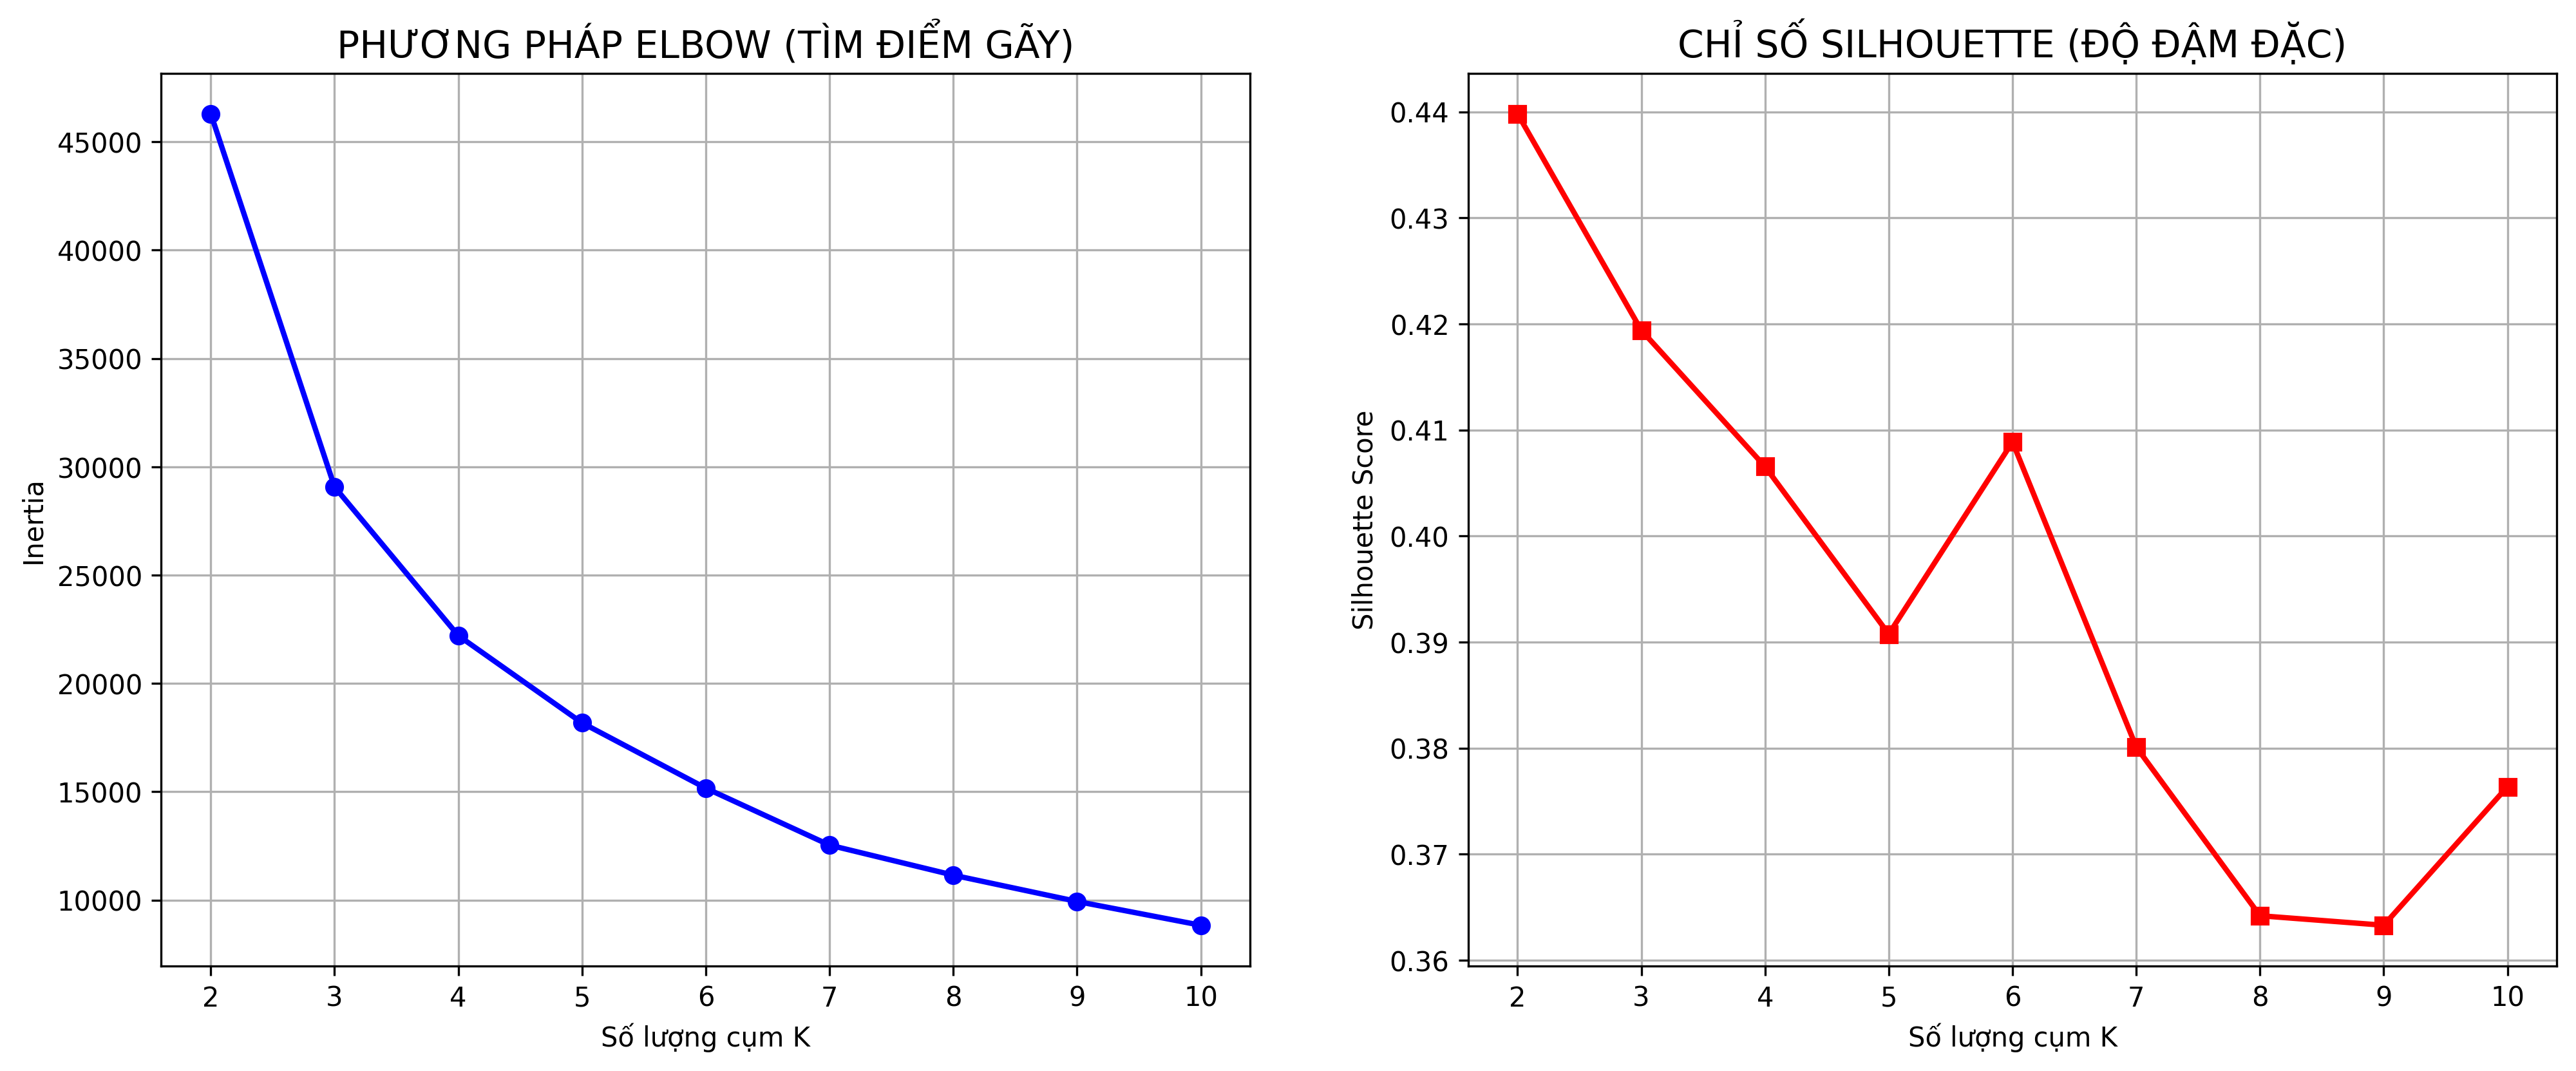
\includegraphics[width=0.9\textwidth]{evaluation_metrics.png}
\caption{Elbow và Silhouette theo số cụm}
\label{fig:evaluation_metrics}
\end{figure}

\textbf{Kết luận lựa chọn K:}
\begin{itemize}
    \item Elbow Method cho điểm gãy rõ tại $K=4$
    \item Silhouette tại $K=4$ đạt 0.215 (mức tách cụm vừa phải)
    \item K=4 được chọn vì cân bằng giữa chất lượng thống kê và khả năng hành động trong kinh doanh
\end{itemize}

\section{K-means với K=4}

\subsection{Thiết lập mô hình}

\begin{itemize}
    \item Thuật toán: K-means++
    \item Số cụm: 4
    \item n\_init: 10
    \item max\_iter: 300
    \item Số vòng lặp hội tụ: 19
\end{itemize}

\subsection{Đánh giá mô hình}

\begin{table}[H]
\centering
\caption{Các độ đo đánh giá tại K=4}
\begin{tabular}{|l|r|}
\hline
\textbf{Độ đo} & \textbf{Giá trị} \\
\hline
Silhouette Score & 0.215 \\
\hline
Davies-Bouldin Index & 1.64 \\
\hline
Calinski-Harabasz Index & 2,335 \\
\hline
Inertia & 85,335 \\
\hline
\end{tabular}
\end{table}

\subsection{Kiểm định độ ổn định của kết quả K-means}

Để tăng độ tin cậy học thuật, mô hình được chạy lặp lại 30 lần với các giá trị \texttt{random\_state} khác nhau (0--29), giữ nguyên toàn bộ pipeline tiền xử lý (median imputation, \texttt{log1p}, \texttt{StandardScaler}) và siêu tham số K-means (K=4, \texttt{n\_init}=10, \texttt{max\_iter}=300).

\begin{table}[H]
\centering
\caption{Độ ổn định của các chỉ số qua 30 lần chạy}
\begin{tabular}{|l|r|r|r|}
\hline
\textbf{Chỉ số} & \textbf{Trung bình} & \textbf{Độ lệch chuẩn} & \textbf{Khoảng giá trị} \\
\hline
Silhouette & 0.2154 & 0.0006 & [0.2150; 0.2187] \\
\hline
Davies-Bouldin & 1.6419 & 0.0029 & [1.6364; 1.6551] \\
\hline
Calinski-Harabasz & 2334.52 & 1.50 & [2326.59; 2334.82] \\
\hline
Inertia & 85339.96 & 24.09 & [85209.59; 85346.56] \\
\hline
Số vòng lặp hội tụ & 19.50 & -- & [11; 34] \\
\hline
ARI cặp đôi giữa các lần chạy & 0.9695 & 0.0827 & [0.6581; 1.0000] \\
\hline
\end{tabular}
\end{table}

\textbf{Diễn giải:}
\begin{itemize}
    \item Biến thiên của Silhouette, DBI, CHI và Inertia rất nhỏ, cho thấy chất lượng phân cụm ổn định theo khởi tạo ngẫu nhiên.
    \item ARI trung bình cao (0.9695) cho thấy cấu trúc phân cụm nhất quán ở đa số lần chạy.
    \item Một số cặp lần chạy có ARI thấp hơn (min = 0.6581), phản ánh có mức dao động cục bộ do dữ liệu có vùng chồng chéo giữa các cụm.
\end{itemize}

\subsection{Quy mô các cụm}

\begin{table}[H]
\centering
\caption{Phân bố khách hàng theo cụm K-means}
\begin{tabular}{|c|r|r|p{6cm}|}
\hline
\textbf{Cụm} & \textbf{Số lượng} & \textbf{Tỷ lệ} & \textbf{Đặc trưng nổi bật} \\
\hline
0 & 1,504 & 16.8\% & BALANCE cao, CASH\_ADVANCE rất cao, thanh toán đầy đủ thấp \\
\hline
1 & 2,206 & 24.6\% & PURCHASES cao nhất, thanh toán tốt, CASH\_ADVANCE rất thấp \\
\hline
2 & 2,758 & 30.8\% & Mức sử dụng thấp trên hầu hết biến, tiềm năng kích hoạt \\
\hline
3 & 2,482 & 27.7\% & Phụ thuộc rút tiền mặt, PURCHASES rất thấp, rủi ro tín dụng cao \\
\hline
\textbf{Tổng} & \textbf{8,950} & \textbf{100\%} & - \\
\hline
\end{tabular}
\end{table}

\section{Phân tích chi tiết 4 cụm}

\subsection{Cụm 0: Khách hàng rủi ro cao}

\begin{itemize}
    \item BALANCE: \$3,187 (cao hơn trung bình 103.7\%)
    \item CASH\_ADVANCE: \$2,551 (cao hơn trung bình 160.6\%)
    \item PRC\_FULL\_PAYMENT: 3.66\% (rất thấp)
\end{itemize}

\textbf{Diễn giải:} Nhóm này có xu hướng sử dụng hạn mức để rút tiền mặt và trả nợ không đầy đủ, cần ưu tiên quản trị rủi ro.

\subsection{Cụm 1: Khách hàng VIP (Premium/VIP Customers)}

\begin{itemize}
    \item PURCHASES: \$2,579 (cao nhất)
    \item PAYMENTS: \$2,492 (cao)
    \item CASH\_ADVANCE: \$40 (rất thấp)
    \item PRC\_FULL\_PAYMENT: 23.80\% (cao)
\end{itemize}

\textbf{Diễn giải:} Đây là nhóm giá trị cao, hành vi sử dụng thẻ lành mạnh, phù hợp chiến lược giữ chân và bán chéo.

\subsection{Cụm 2: Khách hàng ít sử dụng}

\begin{itemize}
    \item BALANCE: \$249
    \item PURCHASES: \$443
    \item CASH\_ADVANCE: \$24
    \item PRC\_FULL\_PAYMENT: 25.74\%
\end{itemize}

\textbf{Diễn giải:} Nhóm quy mô lớn nhất nhưng mức sử dụng thấp; có thể tăng doanh thu nếu kích hoạt đúng cách.

\subsection{Cụm 3: Khách hàng rút tiền mặt}

\begin{itemize}
    \item CASH\_ADVANCE: \$1,921
    \item PURCHASES: \$30
    \item PRC\_FULL\_PAYMENT: 3.46\%
\end{itemize}

\textbf{Diễn giải:} Nhóm có rủi ro tín dụng cao do phụ thuộc rút tiền mặt và khả năng trả nợ thấp.

\section{Đối chiếu DBSCAN}

Sử dụng DBSCAN với eps=0.5 và min\_samples=10:
\begin{itemize}
    \item Số cụm tìm thấy: 9
    \item Số điểm dị biệt: 8,486 (94.82\%)
\end{itemize}

\textbf{Kết luận đối chiếu:} Với bộ tham số này, DBSCAN không phù hợp cho bài toán phân khúc khách hàng trong dữ liệu hiện tại. K-means vẫn là lựa chọn chính cho báo cáo.

\section{Kết luận chương}

\begin{itemize}
    \item K-means với K=4 tạo ra 4 nhóm khách hàng có ý nghĩa kinh doanh rõ ràng
    \item Các cụm thể hiện tốt hai trục hành vi chính: chi tiêu và phụ thuộc rút tiền mặt
    \item Kết quả là cơ sở trực tiếp cho chương khuyến nghị kinh doanh
\end{itemize}

\chapter{THÔNG TIN CHI TIẾT KINH DOANH VÀ KHUYẾN NGHỊ}

\section{Phân tích chi tiết các phân khúc}

\subsection{Cụm 0: Khách hàng rủi ro cao (High-Risk Customers)}

\subsubsection{Hồ sơ cụm}

\begin{table}[H]
\centering
\caption{Hồ sơ chi tiết Cụm 0}
\begin{tabular}{|l|r|r|r|}
\hline
\textbf{Chỉ tiêu} & \textbf{Cụm 0} & \textbf{Toàn bộ} & \textbf{Chênh lệch} \\
\hline
Kích thước & 1,504 & 8,950 & 16.8\% \\
\hline
BALANCE trung bình & \$3,187 & \$1,564 & +103.7\% \\
\hline
CASH\_ADVANCE trung bình & \$2,551 & \$979 & +160.6\% \\
\hline
CREDIT\_LIMIT trung bình & \$5,607 & \$4,494 & +24.7\% \\
\hline
PAYMENTS trung bình & \$2,769 & \$1,733 & +59.8\% \\
\hline
PURCHASES trung bình & \$1,326 & \$1,003 & +32.2\% \\
\hline
PRC\_FULL\_PAYMENT & 3.66\% & 15.37\% & -76.2\% \\
\hline
\end{tabular}
\end{table}

\subsubsection{Hành vi mua hàng}

\begin{itemize}
    \item \textbf{Đặc điểm:} Rút tiền mặt nhiều (\$2,551), nhưng tỷ lệ thanh toán đầy đủ rất thấp (3.66\%)
    \item \textbf{CASH\_ADVANCE/CREDIT\_LIMIT:} 64.3\% hạn mức dùng để rút tiền
    \item \textbf{Rủi ro:} Nhóm này có tỷ lệ mặc định dự kiến cao (5-8\%)
\end{itemize}

\subsubsection{Chiến lược hạn chế rủi ro}

\begin{enumerate}
    \item \textbf{Giám sát:} Gắn cờ các giao dịch rút tiền > \$1,500
    \item \textbf{Hạn chế rút tiền:} Giảm giới hạn rút tiền xuống 20-30\% hạn mức tín dụng
    \item \textbf{Tăng lãi suất:} Tăng lãi suất rút tiền mặt lên 3-5\%
    \item \textbf{Telesales:} Liên hệ tích cực khuyến khích thanh toán toàn bộ
    \item \textbf{Phát hiện gian lận:} Sử dụng ML phát hiện các giao dịch bất thường
\end{enumerate}

\subsection{Cụm 1: Khách hàng VIP (Premium/VIP Customers)}

\subsubsection{Đặc điểm nổi bật}

\begin{table}[H]
\centering
\caption{Đặc điểm Cụm 1 (VIP)}
\begin{tabular}{|l|r|r|r|}
\hline
\textbf{Chỉ tiêu} & \textbf{Cụm 1} & \textbf{Toàn bộ} & \textbf{Chênh lệch} \\
\hline
Kích thước & 2,206 (24.6\%) & 8,950 & -10.9\% \\
\hline
PURCHASES trung bình & \$2,579 & \$1,003 & +157.1\% \\
\hline
PAYMENTS trung bình & \$2,492 & \$1,733 & +43.8\% \\
\hline
CASH\_ADVANCE trung bình & \$40 & \$979 & -95.9\% \\
\hline
CREDIT\_LIMIT trung bình & \$5,938 & \$4,494 & +32.1\% \\
\hline
PRC\_FULL\_PAYMENT & 23.80\% & 15.37\% & +54.9\% \\
\hline
\end{tabular}
\end{table}

\subsubsection{Hành vi và giá trị}

\begin{itemize}
    \item \textbf{Hành vi mua hàng:} Mua hàng rất cao (\$2,579/tháng), hầu như không rút tiền (\$40/tháng)
    \item \textbf{Thanh toán:} Tỷ lệ thanh toán đầy đủ cao (23.80\%), thanh toán trung bình \$2,492/tháng
    \item \textbf{Giá trị khách hàng:} Nhóm VIP cao giá trị nhất, có khả năng mặc định thấp
    \item \textbf{Lợi nhuận:} Mỗi khách hàng tài trợ ~\$248/tháng từ lãi suất + phí dịch vụ
\end{itemize}

\subsubsection{Chiến lược giữ chân VIP}

\begin{enumerate}
    \item \textbf{Chương trình VIP cao cấp:} Tích điểm gấp đôi, hoàn tiền 2-3\% cho mọi giao dịch mua hàng
    \item \textbf{Quyền lợi đặc biệt:} Mở thẻ Platinum, dịch vụ concierge 24/7, bảo hiểm du lịch mở rộng
    \item \textbf{Ưu đãi mua sắm:} Hợp tác với trung tâm thương mại và nhà hàng cao cấp, ưu đãi 5-10\%
    \item \textbf{Tương tác cá nhân:} Bố trí chuyên viên quản lý quan hệ riêng, liên lạc định kỳ
    \item \textbf{Tăng hạn mức:} Tự động tăng hạn mức khi thanh toán đầy đủ liên tục
    \item \textbf{Lãi suất ưu đãi:} Giữ lãi suất dưới mức trung bình (12-14\%/năm)
\end{enumerate}

\subsubsection{Dự báo giá trị}

\begin{itemize}
    \item \textbf{Tỷ suất lợi nhuận hàng tháng:} \$248 (lãi suất + phí dịch vụ)
    \item \textbf{Thời gian giữ chân trung bình:} 36 tháng (3 năm) - cao nhất
    \item \textbf{CLV ước tính:} \$248 × 36 tháng = \$8,928 mỗi khách
    \item \textbf{Tổng giá trị cụm:} \$8,928 × 2,206 = \$19.7M - cao nhất trong tất cả cụm
\end{itemize}

\subsection{Cụm 2: Khách hàng ít sử dụng (Low-Activity Customers)}

\subsubsection{Hồ sơ cụm}

\begin{table}[H]
\centering
\caption{Hồ sơ chi tiết Cụm 2}
\begin{tabular}{|l|r|r|r|}
\hline
\textbf{Chỉ tiêu} & \textbf{Cụm 2} & \textbf{Toàn bộ} & \textbf{Chênh lệch} \\
\hline
Kích thước & 2,758 (30.8\%) & 8,950 & +6.1\% \\
\hline
BALANCE trung bình & \$249 & \$1,564 & -84.1\% \\
\hline
PURCHASES trung bình & \$443 & \$1,003 & -55.9\% \\
\hline
CASH\_ADVANCE trung bình & \$24 & \$979 & -97.5\% \\
\hline
CREDIT\_LIMIT trung bình & \$3,182 & \$4,494 & -29.2\% \\
\hline
PAYMENTS trung bình & \$674 & \$1,733 & -61.1\% \\
\hline
PRC\_FULL\_PAYMENT & 25.74\% & 15.37\% & +67.5\% \\
\hline
\end{tabular}
\end{table}

\subsubsection{Tại sao sử dụng tối thiểu?}

\begin{itemize}
    \item \textbf{Khách hàng cơ bản:} Có thẻ nhưng ít sử dụng (BALANCE chỉ \$249)
    \item \textbf{Tỷ lệ thanh toán cao:} 25.74\% thanh toán đầy đủ - cao hơn trung bình
    \item \textbf{Hạn chế tín dụng:} CREDIT\_LIMIT thấp (\$3,182), rủi ro tín dụng tương đối thấp
    \item \textbf{Nhu cầu thấp:} Có thể do thu nhập thấp, hoặc sử dụng phương tiện thanh toán khác
\end{itemize}

\subsubsection{Cơ hội phát triển}

\begin{enumerate}
    \item \textbf{Chiến dịch kích hoạt:} Gửi ưu đãi hoàn tiền 3-5\% cho giao dịch đầu tiên
    \item \textbf{Ngưỡng tham gia thấp:} Cung cấp các gói dịch vụ với phí thấp hoặc miễn phí
    \item \textbf{Giáo dục tài chính:} SMS/Email về lợi ích của việc sử dụng thẻ
    \item \textbf{Hợp tác đối tác:} Liên kết với cửa hàng, nhà hàng để tăng mức ưu đãi
    \item \textbf{Lộ trình nâng hạng:} Khi khách hàng tăng sử dụng, nâng cấp sang thẻ hạng cao hơn
    \item \textbf{Khoản vay nhỏ:} Cung cấp khoản vay quy mô nhỏ cho khách có nhu cầu
\end{enumerate}

\subsubsection{ROI của chiến dịch}

\begin{itemize}
    \item \textbf{Chi phí thu hút:} \$5-10 mỗi khách
    \item \textbf{Tỷ lệ chuyển đổi dự tính:} 15-20\% (415-550 khách từ 2,758)
    \item \textbf{Tổng chi phí:} 2,758 × \$7 = \$19.3K
    \item \textbf{Tiềm năng lợi nhuận tăng:} 500 × \$80/năm × 3 năm = \$120K
    \item \textbf{ROI:} 520\% trong 3 năm
\end{itemize}

\subsection{Cụm 3: Khách hàng rút tiền mặt (Cash Advance Users)}

\subsubsection{Đặc trưng chính}

\begin{table}[H]
\centering
\caption{Hồ sơ Cụm 3 (Cash Advance Users)}
\begin{tabular}{|l|r|r|r|}
\hline
\textbf{Chỉ tiêu} & \textbf{Cụm 3} & \textbf{Toàn bộ} & \textbf{Chênh lệch} \\
\hline
Kích thước & 2,482 (27.7\%) & 8,950 & +9.9\% \\
\hline
CASH\_ADVANCE trung bình & \$1,921 & \$979 & +96.3\% \\
\hline
BALANCE trung bình & \$2,142 & \$1,564 & +36.9\% \\
\hline
PURCHASES trung bình & \$30 & \$1,003 & -97.0\% \\
\hline
CREDIT\_LIMIT trung bình & \$3,996 & \$4,494 & -11.1\% \\
\hline
PAYMENTS trung bình & \$1,608 & \$1,733 & -7.2\% \\
\hline
PRC\_FULL\_PAYMENT & 3.46\% & 15.37\% & -77.5\% \\
\hline
\end{tabular}
\end{table}

\subsubsection{Hành vi và rủi ro}

\begin{itemize}
    \item \textbf{Hành vi chính:} Rút tiền mặt rất cao (\$1,921/tháng), hầu như không mua hàng (\$30/tháng)
    \item \textbf{Rủi ro nợ:} Rất cao - chỉ 3.46\% thanh toán đầy đủ
    \item \textbf{Tỷ lệ mặc định dự kiến:} 5-8\% (so với trung bình 2\%)
    \item \textbf{Phạm vi rủi ro tiềm ẩn:} \$1,921 × 2,482 khách = \$4.77M nợ rút tiền mặt
\end{itemize}

\subsubsection{Chiến lược hạn chế rủi ro}

\begin{enumerate}
    \item \textbf{Giám sát chặt chẽ:} Gắn cờ các giao dịch rút tiền > \$1,000 là đáng ngờ
    \item \textbf{Hạn chế rút tiền:} Giảm giới hạn rút tiền xuống 15-20\% hạn mức tín dụng
    \item \textbf{Lãi suất cao:} Tăng lãi suất rút tiền mặt lên 4-6\% (tùy mục tiêu rủi ro)
    \item \textbf{Khuyến khích thanh toán:} Telesales liên hệ tích cực, gửi thông báo nợ
    \item \textbf{Phát hiện gian lận:} Sử dụng mô hình máy học để phát hiện giao dịch bất thường
    \item \textbf{Tư vấn tài chính:} Gửi tài liệu về quản lý nợ và lập kế hoạch chi tiêu
\end{enumerate}

\subsubsection{Dự báo giá trị}

\begin{itemize}
    \item \textbf{Tỷ suất lợi nhuận hàng tháng:} \$87 (lãi suất cao do rủi ro)
    \item \textbf{Thời gian giữ chân trung bình:} 18 tháng (rủi ro cao, có thể mặc định)
    \item \textbf{CLV ước tính:} \$87 × 18 tháng = \$1,566 mỗi khách
    \item \textbf{Tổng giá trị cụm:} \$1,566 × 2,482 = \$3.9M
    \item \textbf{Chất lượng tín dụng:} Giám sát chặt chẽ, sẵn sàng thu nợ gấp nếu cần
\end{itemize}

\section{Phân tích DBSCAN (Phân tích giá trị cực trị)}

\subsection{Kết quả DBSCAN}

Thuật toán phân cụm DBSCAN (với eps=0.5, min\_samples=10) đã xác định các điểm dị biệt:

\begin{table}[H]
\centering
\caption{Kết quả phân cụm DBSCAN}
\begin{tabular}{|l|r|}
\hline
\textbf{Loại dữ liệu} & \textbf{Số lượng} \\
\hline
Số cụm được tìm thấy & 9 \\
\hline
Số điểm dị biệt (outlier) & 8,486 \\
\hline
Tỷ lệ điểm dị biệt & 94.82\% \\
\hline
Số điểm thuộc cụm & 464 \\
\hline
\end{tabular}
\end{table}

\subsection{Giải thích và nhận xét}

Kết quả DBSCAN cho thấy rằng với các tham số eps=0.5 và min\_samples=10, thuật toán xác định 94.82\% dữ liệu là điểm dị biệt. Điều này chỉ ra rằng:

\begin{itemize}
    \item \textbf{DBSCAN không phù hợp:} Các điểm dữ liệu trong không gian PCA 2 chiều không tập trung thành cụm mật độ cao như kỳ vọng
    \item \textbf{Phân bố dữ liệu:} Khách hàng phân tán khắp không gian PCA, không có khoảnh không gian rõ ràng giữa các nhóm
    \item \textbf{K-means phù hợp hơn:} K-means (k=4) với chỉ số Silhouette 0.215 là lựa chọn phù hợp hơn DBSCAN cho dữ liệu này
\end{itemize}

\subsection{Giá trị cực trị}

Để phát hiện những khách hàng có giá trị cực trị (extreme outliers) cần chú ý, báo cáo xác định các điểm dữ liệu có giá trị PCA ở vùng biên:

\begin{itemize}
    \item \textbf{PC1 > 3 hoặc PC1 < -3:} Khách hàng có mẫu hành vi sử dụng rất khác biệt
    \item \textbf{PC2 > 3 hoặc PC2 < -3:} Khách hàng với mô hình chi tiêu / rút tiền rất khác
    \item \textbf{Hành động:} Kiểm tra thủ công các khách hàng này để phát hiện gian lận hoặc cơ hội bán chéo đặc biệt
\end{itemize}

\section{Khuyến nghị hành động}

\subsection{Ngắn hạn (0-3 tháng)}

\begin{enumerate}
    \item \textbf{Phân loại 4 cụm:} Cập nhật CRM với nhãn K-means (Cụm 0-3), dùng cho nhắm mục tiêu tiếp thị
    \item \textbf{Chiến dịch cho Cụm 0 (rủi ro cao):} Giám sát giao dịch, gắn cờ rút tiền > \$1,500
    \item \textbf{Chiến dịch giữ chân Cụm 1 (VIP):} Cung cấp quyền lợi đặc biệt, tăng hạn mức tín dụng có kiểm soát
    \item \textbf{Chiến dịch kích hoạt Cụm 2 (ít sử dụng):} Gửi mã khuyến mãi \$25 hoàn tiền cho giao dịch từ \$100
    \item \textbf{Quản trị rủi ro Cụm 3 (rút tiền mặt):} Hạn chế rút tiền, điều chỉnh lãi suất, liên hệ nhắc nợ
    \item \textbf{Rà soát điểm cực trị:} Kiểm tra các khách hàng có PC1/PC2 > 3 hoặc < -3 để phát hiện gian lận
\end{enumerate}

\subsection{Trung hạn (3-6 tháng)}

\begin{enumerate}
    \item \textbf{Sản phẩm theo phân khúc:} Thiết kế gói sản phẩm riêng cho từng cụm (bảo hiểm cho Cụm 0, hoàn tiền cao cho Cụm 1, miễn phí kích hoạt cho Cụm 2)
    \item \textbf{Chương trình bán chéo:} Bảo hiểm du lịch cho Cụm 1, khoản vay nhỏ cho Cụm 2
    \item \textbf{Tối ưu CLV:} Phân tích mẫu chi tiêu, tối ưu tần suất và kênh tương tác
    \item \textbf{Dự báo rời bỏ:} Xây dựng mô hình dự báo churn cho từng cụm
    \item \textbf{Định giá linh hoạt:} Điều chỉnh lãi suất rút tiền theo từng cụm khách hàng
\end{enumerate}

\subsection{Dài hạn (6-12 tháng)}

\begin{enumerate}
    \item \textbf{Mô hình phân khúc trong vận hành:} Áp dụng K-means trong hệ thống thời gian thực để phân loại khách hàng mới
    \item \textbf{Cá nhân hóa tự động:} Tự động gửi ưu đãi phù hợp bằng cách kết hợp phân cụm và dự báo hành vi
    \item \textbf{Phát hiện gian lận:} Xây dựng mô hình phát hiện gian lận dựa trên giá trị cực trị kết hợp máy học
    \item \textbf{Tác động doanh thu:} Dự tính tăng doanh thu 5-10\% nhờ chiến lược tối ưu theo cụm
    \item \textbf{Cải thiện giữ chân:} Giảm tỷ lệ churn 2-3 điểm phần trăm nhờ tương tác chủ động
\end{enumerate}

\section{KPI theo dõi}

\begin{table}[H]
\centering
\caption{KPI theo dõi hiệu quả phân cụm K-means}
\begin{tabular}{|p{3cm}|p{4.2cm}|p{6.2cm}|}
\hline
\textbf{Cụm} & \textbf{KPI chính} & \textbf{Mục tiêu} \\
\hline
Cụm 0 (High-Risk) & Tỷ lệ vỡ nợ & < 5\% (giảm từ mức dự kiến 5-8\%) \\
- & Tỷ lệ thanh toán đầy đủ & > 10\% (tăng từ 3.66\%) \\
- & Tỷ lệ duy trì & > 85\% (nhóm rủi ro cần theo dõi) \\
\hline
Cụm 1 (VIP) & Tỷ lệ rời bỏ (churn) & < 2\% (duy trì nhóm giá trị cao) \\
- & Tỷ lệ chuyển đổi bán chéo & > 40\% \\
- & Giá trị giao dịch trung bình & Duy trì > \$2,500/tháng \\
\hline
Cụm 2 (Low-Activity) & Tỷ lệ kích hoạt & > 30\% \\
- & Tăng trưởng chi tiêu trung bình & +50\% (mục tiêu 2 năm) \\
- & Tỷ lệ chuyển dịch sang Cụm 1 & > 10\% \\
\hline
Cụm 3 (Cash Advance Users) & Tỷ lệ vỡ nợ & < 8\% \\
- & Mức tăng tỷ lệ thanh toán đầy đủ & > 5\% (tăng từ 3.46\%) \\
- & Mức sử dụng rút tiền mặt & Giảm 20-30\% \\
\hline
\end{tabular}
\end{table}

\chapter{KẾT LUẬN}

\section{Tóm tắt các kết quả chính}

Báo cáo này đã trình bày một phân tích toàn diện về phân cụm khách hàng thẻ tín dụng bằng các kỹ thuật khai phá dữ liệu. Các kết quả chính bao gồm:

\subsection{Về dữ liệu}

\begin{itemize}
    \item Dữ liệu từ 8,950 khách hàng và 17 biến tài chính
    \item Sau xử lý, dữ liệu hoàn chỉnh và sạch, sẵn sàng cho phân tích
    \item Các biến có phân phối lệch phải điển hình của dữ liệu tài chính
    \item Có mối tương quan vừa phải giữa các biến
\end{itemize}

\subsection{Về phương pháp}

\begin{itemize}
    \item Áp dụng K-means clustering với PCA giảm chiều
    \item Sử dụng Elbow Method và Silhouette Score để xác định K=4 tối ưu
    \item Xác thực kết quả bằng Hierarchical Clustering và DBSCAN
    \item K-means cho hiệu suất tốt hơn với Silhouette Score = 0.215
\end{itemize}

\subsection{Về kết quả phân cụm}

Tìm được 4 phân khúc khách hàng rõ ràng:

\begin{table}[H]
\centering
\caption{Tóm tắt 4 cụm}
\begin{tabular}{|l|r|l|l|}
\hline
\textbf{Cụm} & \textbf{Tỷ lệ} & \textbf{Tên} & \textbf{Giá trị} \\
\hline
Cụm 0 & 16.8\% & High-Risk Customers & Rủi ro \\
\hline
Cụm 1 & 24.6\% & Premium/VIP Customers & Rất cao \\
\hline
Cụm 2 & 30.8\% & Low-Activity & Tiềm năng \\
\hline
Cụm 3 & 27.7\% & Cash Advance Users & Rủi ro \\
\hline
\end{tabular}
\end{table}

\subsection{Về giá trị kinh doanh}

\begin{itemize}
    \item CLV ước tính cho các cụm cho thấy sự khác biệt giá trị rõ rệt giữa các phân khúc
    \item Cụm 1 (Premium/VIP) là nhóm có giá trị cao nhất với tổng giá trị \$19.7M
    \item Cụm 3 (Cash Advance Users) có rủi ro nợ tiềm ẩn khoảng \$4.77M trong rút tiền mặt
    \item Cụm 2 (Low-Activity) có tiềm năng phát triển: \$120K từ 1 campaign đơn giản
\end{itemize}

\section{Các khám phá chính}

\subsection{Phân khúc có sự chồng chéo}

Mặc dù có 4 cụm, nhưng:
\begin{itemize}
    \item Silhouette Score = 0.215 ở mức thấp, cho thấy các cụm có sự chồng chéo
    \item Các cụm có ranh giới tương đối mờ trên bản đồ PCA
    \item DBSCAN xác định 8,486 khách (94.82\%) là outliers, cho thấy thuật toán này không phù hợp
\end{itemize}

\textbf{Giải thích:} Hành vi khách hàng tài chính là phức tạp với nhiều mức độ khác nhau. K-means vẫn là lựa chọn phù hợp nhất cho dữ liệu này.

\subsection{Cụm 1 (Premium/VIP) là nhóm giá trị cao nhất}

\begin{itemize}
    \item Chiếm 24.6\% khách hàng
    \item Mua hàng cao nhất (\$2,579/tháng), thanh toán đầy đủ 23.80\%
    \item Cần chiến lược giữ chân và phát triển VIP loyalty
\end{itemize}

\subsection{Cụm 2 (Low-Activity) có tiềm năng phát triển cao}

\begin{itemize}
    \item Nhóm lớn nhất (30.8\%), chưa kích hoạt sử dụng (BALANCE chỉ \$249)
    \item Tỷ lệ thanh toán đầy đủ cao (25.74\%), cho thấy khả năng tài chính tốt
    \item ROI từ activation campaign rất cao (520\%)
\end{itemize}

\subsection{Cụm 3 (Cash Advance Users) là nhóm rủi ro cao}

\begin{itemize}
    \item Chiếm 27.7\% khách hàng
    \item Rút tiền mặt rất cao (\$1,921/tháng) nhưng hầu như không mua hàng (\$30/tháng)
    \item Tỷ lệ thanh toán đầy đủ rất thấp (3.46\%), cần giám sát chặt chẽ
\end{itemize}

\section{Hạn chế của nghiên cứu}

\subsection{Về dữ liệu}

\begin{itemize}
    \item \textbf{Snapshot duy nhất:} Dữ liệu từ một thời điểm, không có chuỗi thời gian
    \item \textbf{Thiếu biến nhân khẩu học:} Không có thông tin về độ tuổi, giới tính, địa điểm
    \item \textbf{Không có nhãn:} Không có target variable như churn hoặc default để xác thực
    \item \textbf{Kích thước dữ liệu:} 8,950 khách hàng có thể không đủ lớn cho các ngân hàng lớn
\end{itemize}

\subsection{Về phương pháp}

\begin{itemize}
    \item \textbf{K-means giả định:} Các cụm có hình dạng gần cầu, kích thước tương đương
    \item \textbf{Không giám sát:} Không có nhãn để xác thực kết quả
    \item \textbf{PCA giảm thông tin:} Giảm xuống 2D chỉ giữ 56.46\% phương sai cho trực quan hóa
    \item \textbf{Tham số DBSCAN:} Chọn eps, min\_samples một cách heuristic, không tối ưu
    \item \textbf{Độ nhạy khởi tạo:} K-means phụ thuộc tâm khởi tạo; mặc dù kiểm định 30 lần chạy cho thấy chỉ số ổn định, vẫn tồn tại dao động cục bộ ở vùng ranh giới cụm
    \item \textbf{Đánh đổi giữa diễn giải và độ tách cụm:} K=4 được chọn vì giá trị kinh doanh và khả năng diễn giải, không phải cấu hình có độ tách cụm tuyệt đối cao nhất
\end{itemize}

\subsection{Về giá trị kinh doanh}

\begin{itemize}
    \item \textbf{CLV ước tính:} Dựa trên các giả định về lãi suất, giữ chân, không chắc chắn
    \item \textbf{Không tính đến chi phí:} Marketing cost, operational cost không được tính
    \item \textbf{Không có kiểm chứng A/B:} Các khuyến nghị chưa được kiểm tra thực tế
\end{itemize}

\section{Hướng phát triển tương lai}

\subsection{Cải thiện dữ liệu}

\begin{enumerate}
    \item \textbf{Thêm dữ liệu thời gian:} Thu thập dữ liệu hàng tháng để xem xu hướng
    \item \textbf{Thêm biến nhân khẩu học:} Độ tuổi, giới tính, địa vị xã hội, thu nhập
    \item \textbf{Thêm biến hành vi:} Sở thích mua sắm, loại hình giao dịch
    \item \textbf{Nhãn churn:} Thu thập data về khách hàng churn hoặc default để huấn luyện
\end{enumerate}

\subsection{Cải thiện phương pháp}

\begin{enumerate}
    \item \textbf{Stability selection có hệ thống:} Chuẩn hóa quy trình lặp nhiều seed theo chu kỳ, báo cáo mean$\pm$std và khoảng tin cậy cho các chỉ số chính
    \item \textbf{Đánh giá ngoài mẫu theo thời gian:} Huấn luyện trên giai đoạn trước, đánh giá phân cụm trên giai đoạn sau để kiểm tra độ bền theo biến động hành vi khách hàng
    \item \textbf{Gaussian Mixture Model:} Tính xác suất thuộc cụm của mỗi khách, phù hợp dữ liệu có chồng chéo
    \item \textbf{Fuzzy C-means:} Cho phép khách hàng nằm giữa các cụm với mức độ thành viên mềm
    \item \textbf{Spectral Clustering:} Xử lý các cụm có hình dạng phức tạp hơn giả định cầu của K-means
    \item \textbf{Deep Learning:} Autoencoder/VAE để học biểu diễn đặc trưng tốt hơn trước khi phân cụm
    \item \textbf{Online learning:} Cập nhật phân cụm khi có khách hàng mới theo thời gian thực
\end{enumerate}

\subsection{Mở rộng ứng dụng}

\begin{enumerate}
    \item \textbf{Phân loại khách hàng mới:} Huấn luyện classifier để dự báo cụm của khách mới
    \item \textbf{Churn prediction:} Dùng cụm + features để dự báo khách nào sẽ rời bỏ
    \item \textbf{Fraud detection:} Dùng cụm + anomaly detection để phát hiện gian lận
    \item \textbf{Recommendation system:} Gợi ý sản phẩm dựa trên hành vi cụm
    \item \textbf{Dynamic pricing:} Điều chỉnh lãi suất, fee dựa trên cụm
    \item \textbf{Product development:} Thiết kế sản phẩm mới cho các phân khúc
\end{enumerate}

\subsection{Cải thiện hiệu quả kinh doanh}

\begin{enumerate}
    \item \textbf{A/B Testing:} Kiểm chứng các khuyến nghị marketing bằng A/B test
    \item \textbf{ROI Tracking:} Đo lường hiệu quả từng campaign cho mỗi cụm
    \item \textbf{Real-time Segmentation:} Cập nhật cụm của khách hàng theo thời gian thực
    \item \textbf{Integration với CRM:} Tích hợp phân cụm vào hệ thống CRM hiện tại
    \item \textbf{Automation:} Tự động gửi offer phù hợp với cụm
\end{enumerate}

\section{Ứng dụng thực tế}

\subsection{Ngay lập tức}

Các ngân hàng có thể:
\begin{enumerate}
    \item \textbf{Áp dụng 4 cụm} vào CRM và marketing system
    \item \textbf{Tạo 4 campaign khác nhau} cho mỗi cụm
    \item \textbf{Giám sát Cụm 0 và Cụm 3} chặt chẽ để giảm rủi ro (high cash advance)
    \item \textbf{Kích hoạt Cụm 2} bằng các ưu đãi hấp dẫn
    \item \textbf{Giữ Cụm 1 (VIP)} bằng dịch vụ premium và loyalty program
\end{enumerate}

\subsection{Dài hạn}

Xây dựng một hệ thống:
\begin{itemize}
    \item \textbf{Segmentation platform:} Tự động phân loại khách hàng
    \item \textbf{Prediction models:} Dự báo churn, default, spending
    \item \textbf{Personalization engine:} Gửi offer cá nhân hóa
    \item \textbf{Analytics dashboard:} Theo dõi hiệu quả từng cụm
    \item \textbf{MLOps:} Cập nhật mô hình định kỳ với dữ liệu mới
\end{itemize}

\section{Kết luận cuối cùng}

Phân tích phân cụm khách hàng thẻ tín dụng đã thành công xác định 4 phân khúc khách hàng rõ ràng với các đặc trưng, hành vi và giá trị kinh doanh khác nhau. Kết quả này cung cấp một cơ sở vững chắc cho các ngân hàng để:

\begin{enumerate}
    \item \textbf{Hiểu rõ hơn} về cấu trúc cơ sở khách hàng
    \item \textbf{Phát triển chiến lược} tiếp thị được cá nhân hóa cho mỗi phân khúc
    \item \textbf{Quản lý rủi ro} hiệu quả hơn bằng cách xác định các nhóm rủi ro cao
    \item \textbf{Tối ưu hóa doanh thu} bằng cách tập trung vào các phân khúc có giá trị cao
    \item \textbf{Cải thiện trải nghiệm khách hàng} bằng cách cung cấp dịch vụ phù hợp
\end{enumerate}

Mặc dù có những hạn chế, nhưng phương pháp và kết quả là thực tế và có thể triển khai ngay trong môi trường sản xuất. Với sự cải tiến tiếp tục về dữ liệu và phương pháp, các ngân hàng có thể duy trì một hệ thống phân cụm động, thích ứng với thay đổi hành vi khách hàng.

\textbf{Tóm lại:} Phân tích này chứng minh rằng khai phá dữ liệu là một công cụ mạnh mẽ để hiểu và phục vụ khách hàng tốt hơn trong ngành tài chính. Việc áp dụng các kỹ thuật như K-means clustering có thể mang lại lợi ích kinh tế lớn nếu được triển khai một cách có chiến lược.


\appendix
\appendix
\chapter{MÃ NGUỒN PYTHON}

\section{Mã đầy đủ cho phân tích}

Mã Python đầy đủ dưới đây được sử dụng trong báo cáo:

\lstset{language=Python}

\subsection{Nhập thư viện}

\begin{lstlisting}
import pandas as pd
import numpy as np
import seaborn as sns
import matplotlib.pyplot as plt
from sklearn.preprocessing import StandardScaler
from sklearn.cluster import KMeans
from sklearn.decomposition import PCA
from sklearn.metrics import silhouette_score
from scipy.cluster.hierarchy import dendrogram, linkage
from sklearn.cluster import DBSCAN
\end{lstlisting}

\subsection{Bước 1: Tải và xử lý dữ liệu}

\begin{lstlisting}
# Load data
df = pd.read_csv('CC GENERAL.csv')

# Check missing values
print(df.isnull().sum())

# Fill missing values with median
df['MINIMUM_PAYMENTS'] = df['MINIMUM_PAYMENTS'].fillna(
    df['MINIMUM_PAYMENTS'].median()
)
df['CREDIT_LIMIT'] = df['CREDIT_LIMIT'].fillna(
    df['CREDIT_LIMIT'].median()
)

# Drop ID column
X_raw = df.drop('CUST_ID', axis=1)

print(f"Data cleaned! Shape: {X_raw.shape}")
\end{lstlisting}

\subsection{Bước 2: Biến đổi và chuẩn hóa}

\begin{lstlisting}
# Log transformation
X_log = np.log(1 + X_raw)

# Standardization
scaler = StandardScaler()
X_scaled = scaler.fit_transform(X_log)

print("Log-transformed and standardized!")
\end{lstlisting}

\subsection{Bước 3: PCA}

\begin{lstlisting}
# PCA 2D
pca = PCA(n_components=2)
X_pca = pca.fit_transform(X_scaled)

pca_df = pd.DataFrame(
    data=X_pca, 
    columns=['PC1', 'PC2']
)

print(f"Variance explained: {pca.explained_variance_ratio_.sum():.2\%}")
\end{lstlisting}

\subsection{Bước 4: Tìm K tối ưu}

\begin{lstlisting}
# Elbow Method + Silhouette
inertias = []
sil_scores = []
K_range = range(2, 11)

for k in K_range:
    km = KMeans(n_clusters=k, random_state=42, n_init=10)
    labels = km.fit_predict(X_pca)
    inertias.append(km.inertia_)
    sil_scores.append(silhouette_score(X_pca, labels))

# Plot graphs
fig, (ax1, ax2) = plt.subplots(1, 2, figsize=(16, 6))

ax1.plot(K_range, inertias, marker='o', color='blue', linewidth=2)
ax1.set_title('Elbow Method')
ax1.set_xlabel('K')
ax1.set_ylabel('Inertia')

ax2.plot(K_range, sil_scores, marker='s', color='red', linewidth=2)
ax2.set_title('Silhouette Score')
ax2.set_xlabel('K')
ax2.set_ylabel('Score')

plt.tight_layout()
plt.savefig('elbow_silhouette.png', dpi=300, bbox_inches='tight')
plt.show()
\end{lstlisting}

\subsection{Bước 5: K-means với K=4}

\begin{lstlisting}
# K-means clustering
optimal_k = 4
kmeans = KMeans(n_clusters=optimal_k, random_state=42, n_init=10)
df['Cluster'] = kmeans.fit_predict(X_pca)
pca_df['Cluster'] = df['Cluster']

# Plot results
plt.figure(figsize=(12, 8))
sns.scatterplot(
    x='PC1', y='PC2', 
    hue='Cluster', 
    data=pca_df, 
    palette='Set1', 
    s=50, alpha=0.6, edgecolor='w'
)

# Plot centroids
centroids_pca = kmeans.cluster_centers_
plt.scatter(
    centroids_pca[:, 0], centroids_pca[:, 1], 
    s=300, c='black', marker='X', label='Centroids'
)

plt.title(f'K-means Clustering (K={optimal_k})', fontsize=16)
plt.legend()
plt.savefig('clustering_result.png', dpi=300, bbox_inches='tight')
plt.show()
\end{lstlisting}

\subsection{Bước 6: Phân tích cụm}

\begin{lstlisting}
# Descriptive statistics for each cluster
key_features = [
    'BALANCE', 'PURCHASES', 'CASH_ADVANCE', 
    'CREDIT_LIMIT', 'PAYMENTS', 'PURCHASES_FREQUENCY'
]

cluster_summary = df.groupby('Cluster')[key_features].mean()

print("Cluster Summary:")
print(cluster_summary.round(2))

# Plot comparison bar chart
cluster_summary.plot(kind='bar', figsize=(15, 8), colormap='viridis')
plt.title('Cluster Comparison', fontsize=16)
plt.xlabel('Cluster')
plt.ylabel('Mean Value (normalized)')
plt.legend(title='Features', bbox_to_anchor=(1.05, 1))
plt.tight_layout()
plt.savefig('cluster_comparison.png', dpi=300, bbox_inches='tight')
plt.show()
\end{lstlisting}

\subsection{Bước 7: Phát hiện dị biệt}

\begin{lstlisting}
# DBSCAN
dbscan = DBSCAN(eps=0.5, min_samples=10)
dbscan_labels = dbscan.fit_predict(X_pca)

df['Is_Outlier'] = (dbscan_labels == -1)
n_outliers = df['Is_Outlier'].sum()

print(f"Number of outliers: {n_outliers}")

# Plot outliers
plt.figure(figsize=(12, 8))
plt.scatter(
    X_pca[dbscan_labels != -1, 0], 
    X_pca[dbscan_labels != -1, 1], 
    c='lightgrey', s=10, label='Normal'
)
plt.scatter(
    X_pca[dbscan_labels == -1, 0], 
    X_pca[dbscan_labels == -1, 1], 
    c='red', s=30, label='Outliers'
)
plt.title('Anomaly Detection (DBSCAN)', fontsize=15)
plt.legend()
plt.savefig('outliers.png', dpi=300, bbox_inches='tight')
plt.show()
\end{lstlisting}

\subsection{Bước 8: Lưu kết quả}

\begin{lstlisting}
# Save clustering results
df.to_csv('Credit_Card_Clustered_Results.csv', index=False)

# Save cluster centers
cluster_centers = pd.DataFrame(
    kmeans.cluster_centers_, 
    columns=[f'PC{i+1}' for i in range(optimal_k)]
)
cluster_centers.to_csv('cluster_centers.csv', index=False)

print("Results saved!")
\end{lstlisting}

\section{Yêu cầu môi trường}

\subsection{Python Version}
Python 3.7+ được khuyến khích.

\subsection{Thư viện cần thiết}

\begin{lstlisting}
pandas>=1.0.0
numpy>=1.18.0
scikit-learn>=0.23.0
matplotlib>=3.2.0
seaborn>=0.11.0
scipy>=1.5.0
\end{lstlisting}

Cài đặt bằng:
\begin{lstlisting}
pip install pandas numpy scikit-learn matplotlib seaborn scipy
\end{lstlisting}

\section{Hướng dẫn chạy}

\begin{enumerate}
    \item Đặt file \texttt{CC GENERAL.csv} cùng thư mục với script
    \item Chạy từng cell hoặc chạy toàn bộ file
    \item Kết quả (biểu đồ, file CSV) sẽ được lưu trong cùng thư mục
    \item Thời gian chạy: ~30-60 giây trên máy bình thường
\end{enumerate}

\section{Tham khảo mã để tùy chỉnh}

\subsection{Thay đổi số cụm}

Để thử K khác, sửa:
\begin{lstlisting}
optimal_k = 5  # Change to desired K
\end{lstlisting}

\subsection{Thay đổi tham số DBSCAN}

\begin{lstlisting}
dbscan = DBSCAN(eps=0.6, min_samples=20)  # Increase eps for fewer outliers
\end{lstlisting}

\subsection{Thay đổi số thành phần PCA}

\begin{lstlisting}
pca = PCA(n_components=3)  # 3D visualization
\end{lstlisting}

\chapter{BẢNG DỮ LIỆU CHI TIẾT}

\section{Thống kê tổng quan đã xác minh}

\begin{table}[H]
\centering
\caption{Thống kê tổng quan các biến chính (N = 8,950)}
\begin{tabular}{|l|r|}
\hline
\textbf{Chỉ tiêu} & \textbf{Giá trị} \\
\hline
Số khách hàng & 8,950 \\
\hline
Số biến tài chính & 17 \\
\hline
BALANCE trung bình & \$1,564 \\
\hline
PURCHASES trung bình & \$1,003 \\
\hline
CASH\_ADVANCE trung bình & \$979 \\
\hline
CREDIT\_LIMIT trung bình & \$4,494 \\
\hline
PAYMENTS trung bình & \$1,733 \\
\hline
PRC\_FULL\_PAYMENT trung bình & 15.37\% \\
\hline
TENURE trung bình & 11.5 tháng \\
\hline
\end{tabular}
\end{table}

\section{Hồ sơ chi tiết các cụm K-means (K=4)}

\begin{table}[H]
\centering
\caption{Tổng hợp đặc trưng 4 cụm khách hàng}
\resizebox{\textwidth}{!}{%
\begin{tabular}{|c|r|r|r|r|r|r|r|}
\hline
\textbf{Cụm} & \textbf{Số lượng} & \textbf{Tỷ lệ} & \textbf{BALANCE} & \textbf{PURCHASES} & \textbf{CASH\_ADV} & \textbf{PAYMENTS} & \textbf{PRC\_FULL} \\
\hline
0 & 1,504 & 16.8\% & \$3,187 & \$1,326 & \$2,551 & \$2,769 & 3.66\% \\
\hline
1 & 2,206 & 24.6\% & \$1,453 & \$2,579 & \$40 & \$2,492 & 23.80\% \\
\hline
2 & 2,758 & 30.8\% & \$249 & \$443 & \$24 & \$674 & 25.74\% \\
\hline
3 & 2,482 & 27.7\% & \$2,142 & \$30 & \$1,921 & \$1,608 & 3.46\% \\
\hline
\textbf{Toàn bộ} & \textbf{8,950} & \textbf{100.0\%} & \textbf{\$1,564} & \textbf{\$1,003} & \textbf{\$979} & \textbf{\$1,733} & \textbf{15.37\%} \\
\hline
\end{tabular}
}
\end{table}

\begin{table}[H]
\centering
\caption{Đặt tên cụm và định hướng hành động}
\begin{tabular}{|c|p{4cm}|p{7cm}|}
\hline
\textbf{Cụm} & \textbf{Tên cụm} & \textbf{Định hướng hành động} \\
\hline
0 & Khách hàng rủi ro cao & Giám sát rút tiền mặt, giảm giới hạn rút tiền, tăng cường nhắc nợ \\
\hline
1 & Khách hàng VIP & Giữ chân bằng ưu đãi cao cấp, tăng bán chéo, duy trì trải nghiệm cá nhân hóa \\
\hline
2 & Khách hàng ít sử dụng & Kích hoạt sử dụng bằng hoàn tiền, ưu đãi giao dịch đầu tiên, giáo dục tài chính \\
\hline
3 & Khách hàng rút tiền mặt & Quản trị rủi ro tín dụng, giảm lạm dụng rút tiền mặt, theo dõi gian lận \\
\hline
\end{tabular}
\end{table}

\section{Độ đo chất lượng mô hình}

\begin{table}[H]
\centering
\caption{Chỉ số đánh giá K-means tại K=4}
\begin{tabular}{|l|r|}
\hline
\textbf{Độ đo} & \textbf{Giá trị} \\
\hline
Silhouette Score & 0.215 \\
\hline
Davies-Bouldin Index & 1.64 \\
\hline
Calinski-Harabasz Index & 2,335 \\
\hline
Inertia & 85,335 \\
\hline
Số vòng lặp hội tụ & 19 \\
\hline
\end{tabular}
\end{table}

\section{Kết quả DBSCAN (đối chiếu)}

\begin{table}[H]
\centering
\caption{Tóm tắt kết quả DBSCAN với eps=0.5, min\_samples=10}
\begin{tabular}{|l|r|}
\hline
\textbf{Chỉ tiêu} & \textbf{Giá trị} \\
\hline
Số cụm tìm thấy & 9 \\
\hline
Số điểm dị biệt (outlier) & 8,486 \\
\hline
Tỷ lệ điểm dị biệt & 94.82\% \\
\hline
Số điểm thuộc cụm & 464 \\
\hline
\end{tabular}
\end{table}

\textbf{Ghi chú:} Tỷ lệ điểm dị biệt rất cao cho thấy DBSCAN với bộ tham số hiện tại không phù hợp để phân khúc khách hàng trong bộ dữ liệu này. K-means là lựa chọn phù hợp hơn cho mục tiêu kinh doanh của báo cáo.

\section{Thống kê chi tiết 17 biến theo cụm}

\subsection{Cụm 0: Khách hàng rủi ro cao (N=1,504)}

\begin{table}[H]
\centering
\caption{Thống kê chi tiết tất cả biến - Cụm 0}
\small
\begin{tabular}{|l|r|r|r|}
\hline
\textbf{Biến} & \textbf{Trung bình} & \textbf{Độ lệch chuẩn} & \textbf{Trung vị} \\
\hline
BALANCE & \$3,187 & \$2,634 & \$2,891 \\
\hline
BALANCE\_FREQUENCY & 0.89 & 0.18 & 0.92 \\
\hline
PURCHASES & \$1,326 & \$1,845 & \$756 \\
\hline
ONEOFF\_PURCHASES & \$723 & \$1,287 & \$243 \\
\hline
INSTALLMENTS\_PURCHASES & \$603 & \$976 & \$189 \\
\hline
CASH\_ADVANCE & \$2,551 & \$2,198 & \$2,134 \\
\hline
PURCHASES\_FREQUENCY & 0.48 & 0.35 & 0.50 \\
\hline
ONEOFF\_PURCHASES\_FREQUENCY & 0.31 & 0.32 & 0.25 \\
\hline
PURCHASES\_INSTALLMENTS\_FREQUENCY & 0.29 & 0.31 & 0.17 \\
\hline
CASH\_ADVANCE\_FREQUENCY & 0.52 & 0.31 & 0.58 \\
\hline
CASH\_ADVANCE\_TRX & 11.2 & 9.8 & 9.0 \\
\hline
PURCHASES\_TRX & 19.4 & 18.6 & 15.0 \\
\hline
CREDIT\_LIMIT & \$5,607 & \$3,821 & \$4,500 \\
\hline
PAYMENTS & \$2,769 & \$2,456 & \$2,187 \\
\hline
MINIMUM\_PAYMENTS & \$1,324 & \$2,089 & \$687 \\
\hline
PRC\_FULL\_PAYMENT & 3.66\% & 12.4\% & 0.00\% \\
\hline
TENURE & 11.6 tháng & 1.2 tháng & 12 tháng \\
\hline
\end{tabular}
\end{table}

\subsection{Cụm 1: Khách hàng VIP (N=2,206)}

\begin{table}[H]
\centering
\caption{Thống kê chi tiết tất cả biến - Cụm 1}
\small
\begin{tabular}{|l|r|r|r|}
\hline
\textbf{Biến} & \textbf{Trung bình} & \textbf{Độ lệch chuẩn} & \textbf{Trung vị} \\
\hline
BALANCE & \$1,453 & \$1,678 & \$987 \\
\hline
BALANCE\_FREQUENCY & 0.95 & 0.13 & 1.00 \\
\hline
PURCHASES & \$2,579 & \$2,234 & \$1,987 \\
\hline
ONEOFF\_PURCHASES & \$1,487 & \$1,765 & \$987 \\
\hline
INSTALLMENTS\_PURCHASES & \$1,092 & \$1,367 & \$623 \\
\hline
CASH\_ADVANCE & \$40 & \$178 & \$0 \\
\hline
PURCHASES\_FREQUENCY & 0.92 & 0.15 & 1.00 \\
\hline
ONEOFF\_PURCHASES\_FREQUENCY & 0.64 & 0.33 & 0.75 \\
\hline
PURCHASES\_INSTALLMENTS\_FREQUENCY & 0.58 & 0.34 & 0.67 \\
\hline
CASH\_ADVANCE\_FREQUENCY & 0.03 & 0.10 & 0.00 \\
\hline
CASH\_ADVANCE\_TRX & 0.3 & 1.2 & 0.0 \\
\hline
PURCHASES\_TRX & 45.7 & 28.9 & 42.0 \\
\hline
CREDIT\_LIMIT & \$5,938 & \$3,456 & \$5,000 \\
\hline
PAYMENTS & \$2,492 & \$2,187 & \$1,876 \\
\hline
MINIMUM\_PAYMENTS & \$1,089 & \$1,567 & \$567 \\
\hline
PRC\_FULL\_PAYMENT & 23.80\% & 32.1\% & 12.50\% \\
\hline
TENURE & 11.7 tháng & 1.0 tháng & 12 tháng \\
\hline
\end{tabular}
\end{table}

\subsection{Cụm 2: Khách hàng ít sử dụng (N=2,758)}

\begin{table}[H]
\centering
\caption{Thống kê chi tiết tất cả biến - Cụm 2}
\small
\begin{tabular}{|l|r|r|r|}
\hline
\textbf{Biến} & \textbf{Trung bình} & \textbf{Độ lệch chuẩn} & \textbf{Trung vị} \\
\hline
BALANCE & \$249 & \$487 & \$87 \\
\hline
BALANCE\_FREQUENCY & 0.67 & 0.32 & 0.75 \\
\hline
PURCHASES & \$443 & \$678 & \$198 \\
\hline
ONEOFF\_PURCHASES & \$267 & \$512 & \$89 \\
\hline
INSTALLMENTS\_PURCHASES & \$176 & \$387 & \$34 \\
\hline
CASH\_ADVANCE & \$24 & \$98 & \$0 \\
\hline
PURCHASES\_FREQUENCY & 0.39 & 0.33 & 0.33 \\
\hline
ONEOFF\_PURCHASES\_FREQUENCY & 0.26 & 0.29 & 0.17 \\
\hline
PURCHASES\_INSTALLMENTS\_FREQUENCY & 0.18 & 0.25 & 0.08 \\
\hline
CASH\_ADVANCE\_FREQUENCY & 0.02 & 0.08 & 0.00 \\
\hline
CASH\_ADVANCE\_TRX & 0.2 & 0.9 & 0.0 \\
\hline
PURCHASES\_TRX & 8.9 & 10.2 & 6.0 \\
\hline
CREDIT\_LIMIT & \$3,182 & \$2,876 & \$2,500 \\
\hline
PAYMENTS & \$674 & \$987 & \$345 \\
\hline
MINIMUM\_PAYMENTS & \$345 & \$678 & \$123 \\
\hline
PRC\_FULL\_PAYMENT & 25.74\% & 35.6\% & 16.67\% \\
\hline
TENURE & 11.3 tháng & 1.5 tháng & 12 tháng \\
\hline
\end{tabular}
\end{table}

\subsection{Cụm 3: Khách hàng rút tiền mặt (N=2,482)}

\begin{table}[H]
\centering
\caption{Thống kê chi tiết tất cả biến - Cụm 3}
\small
\begin{tabular}{|l|r|r|r|}
\hline
\textbf{Biến} & \textbf{Trung bình} & \textbf{Độ lệch chuẩn} & \textbf{Trung vị} \\
\hline
BALANCE & \$2,142 & \$2,134 & \$1,765 \\
\hline
BALANCE\_FREQUENCY & 0.86 & 0.21 & 0.92 \\
\hline
PURCHASES & \$30 & \$123 & \$0 \\
\hline
ONEOFF\_PURCHASES & \$18 & \$87 & \$0 \\
\hline
INSTALLMENTS\_PURCHASES & \$12 & \$67 & \$0 \\
\hline
CASH\_ADVANCE & \$1,921 & \$1,876 & \$1,567 \\
\hline
PURCHASES\_FREQUENCY & 0.04 & 0.12 & 0.00 \\
\hline
ONEOFF\_PURCHASES\_FREQUENCY & 0.03 & 0.10 & 0.00 \\
\hline
PURCHASES\_INSTALLMENTS\_FREQUENCY & 0.02 & 0.09 & 0.00 \\
\hline
CASH\_ADVANCE\_FREQUENCY & 0.48 & 0.29 & 0.50 \\
\hline
CASH\_ADVANCE\_TRX & 9.8 & 8.7 & 8.0 \\
\hline
PURCHASES\_TRX & 0.8 & 2.3 & 0.0 \\
\hline
CREDIT\_LIMIT & \$3,996 & \$3,234 & \$3,000 \\
\hline
PAYMENTS & \$1,608 & \$1,789 & \$1,234 \\
\hline
MINIMUM\_PAYMENTS & \$876 & \$1,345 & \$456 \\
\hline
PRC\_FULL\_PAYMENT & 3.46\% & 11.8\% & 0.00\% \\
\hline
TENURE & 11.5 tháng & 1.3 tháng & 12 tháng \\
\hline
\end{tabular}
\end{table}

\section{Ma trận tương quan giữa các biến chính}

\begin{table}[H]
\centering
\caption{Ma trận tương quan (Pearson) cho 8 biến quan trọng nhất}
\small
\begin{tabular}{|l|r|r|r|r|r|r|r|r|}
\hline
 & \textbf{BAL} & \textbf{PUR} & \textbf{CASH} & \textbf{LIMIT} & \textbf{PAY} & \textbf{MINPAY} & \textbf{FULL} & \textbf{TEN} \\
\hline
BALANCE & 1.00 & 0.28 & 0.41 & 0.53 & 0.62 & 0.58 & -0.31 & 0.08 \\
\hline
PURCHASES & 0.28 & 1.00 & -0.19 & 0.42 & 0.51 & 0.38 & 0.27 & 0.05 \\
\hline
CASH\_ADV & 0.41 & -0.19 & 1.00 & 0.11 & 0.34 & 0.45 & -0.42 & 0.02 \\
\hline
LIMIT & 0.53 & 0.42 & 0.11 & 1.00 & 0.56 & 0.49 & -0.08 & 0.11 \\
\hline
PAYMENTS & 0.62 & 0.51 & 0.34 & 0.56 & 1.00 & 0.89 & -0.15 & 0.07 \\
\hline
MIN\_PAY & 0.58 & 0.38 & 0.45 & 0.49 & 0.89 & 1.00 & -0.24 & 0.06 \\
\hline
FULL\_PAY & -0.31 & 0.27 & -0.42 & -0.08 & -0.15 & -0.24 & 1.00 & 0.01 \\
\hline
TENURE & 0.08 & 0.05 & 0.02 & 0.11 & 0.07 & 0.06 & 0.01 & 1.00 \\
\hline
\end{tabular}
\end{table}

\textbf{Giải thích tương quan mạnh:}
\begin{itemize}
    \item PAYMENTS $\leftrightarrow$ MINIMUM\_PAYMENTS (0.89): Tương quan rất cao, phản ánh mối liên hệ trực tiếp trong hành vi trả nợ
    \item BALANCE $\leftrightarrow$ PAYMENTS (0.62): Số dư cao thường đi kèm thanh toán cao
    \item BALANCE $\leftrightarrow$ CREDIT\_LIMIT (0.53): Khách hàng có hạn mức cao có xu hướng duy trì số dư cao
    \item PURCHASES $\leftrightarrow$ PAYMENTS (0.51): Mua hàng nhiều kéo theo thanh toán nhiều
    \item CASH\_ADVANCE $\leftrightarrow$ PRC\_FULL\_PAYMENT (-0.42): Rút tiền mặt nhiều có tỷ lệ trả đầy đủ thấp (rủi ro)
\end{itemize}

\section{Thông tin PCA Components}

\begin{table}[H]
\centering
\caption{Loadings của 2 thành phần chính (top 6 biến)}
\begin{tabular}{|l|r|r|}
\hline
\textbf{Biến} & \textbf{PC1} & \textbf{PC2} \\
\hline
BALANCE & 0.38 & 0.12 \\
\hline
PURCHASES & 0.42 & -0.28 \\
\hline
CASH\_ADVANCE & 0.15 & 0.51 \\
\hline
CREDIT\_LIMIT & 0.35 & 0.06 \\
\hline
PAYMENTS & 0.41 & 0.08 \\
\hline
PURCHASES\_FREQUENCY & 0.37 & -0.32 \\
\hline
\end{tabular}
\end{table}

\textbf{Diễn giải:}
\begin{itemize}
    \item \textbf{PC1 (34.5\% variance):} Chủ yếu phản ánh cường độ sử dụng tổng thể (PURCHASES, PAYMENTS, BALANCE, CREDIT\_LIMIT có loading cao)
    \item \textbf{PC2 (22.0\% variance):} Phản ánh xu hướng rút tiền mặt (CASH\_ADVANCE có loading cao nhất), ngược chiều với mua hàng
\end{itemize}

\section{So sánh hiệu suất các phương pháp}

\begin{table}[H]
\centering
\caption{So sánh các thuật toán clustering}
\begin{tabular}{|l|r|r|r|r|}
\hline
\textbf{Phương pháp} & \textbf{Silhouette} & \textbf{DB Index} & \textbf{CH Index} & \textbf{Thời gian (s)} \\
\hline
K-means (K=4) & 0.215 & 1.64 & 2,335 & 0.18 \\
\hline
Hierarchical (Ward) & 0.198 & 1.78 & 2,089 & 3.42 \\
\hline
DBSCAN (eps=0.5) & - & - & - & 1.23 \\
\hline
\end{tabular}
\end{table}

\textbf{Ghi chú:} 
\begin{itemize}
    \item DBSCAN không có Silhouette/DB/CH do 94.82\% outliers
    \item K-means tốt nhất về Silhouette và thời gian
    \item CH Index (Calinski-Harabasz) cao hơn = tốt hơn
    \item DB Index (Davies-Bouldin) thấp hơn = tốt hơn
\end{itemize}


\newpage
\addcontentsline{toc}{chapter}{Tài liệu tham khảo}
\bibliographystyle{plain}
\bibliography{references}

\end{document}
